\documentclass[12pt]{article}
\usepackage{amsmath,amssymb,amsfonts}
\usepackage{geometry}
\usepackage[most]{tcolorbox}
\geometry{margin=1in}
\usepackage{graphicx} % Required for inserting images 
\graphicspath{{figures/}}
\usepackage{physics}
\usepackage{hyperref}
\usepackage{url}
\usepackage{booktabs}
\usepackage{multirow}
\usepackage[numbers,sort&compress]{natbib}
\usepackage{pgfplotstable}
\usepackage{longtable}
\usepackage{float}
\pgfplotstableread[col sep=comma]{sft_benchmarks.csv}\sftdata
\usepackage{siunitx}
\usepackage{geometry}
\usepackage{hyperref}
\usepackage{bm}
\geometry{margin=1in}
\sisetup{detect-all=true}

\title{
\textbf{Spacefield Transformation I:}\\
\textbf{A Geometric Closure Framework for Cosmological Mass,}\\
\textbf{Confinement Scale, and Expansion Dynamics}
}

\author{
Joshua Chukwuemeke Egbon\\
\small Spacefield Transformation Technologies Ltd, United Kingdom\\
\small \texttt{joshua@spacefieldtech.com}
}

\date{}

\begin{document}
\maketitle

\begin{abstract}

Within the minimal SFT closure framework, the global mass--curvature
configuration is constrained by a compactness-saturation condition and
a projected mass--area partition. The dimensionless closure structure
determines the relative confinement geometry, while the absolute
cosmological scale is specified by the baseline confinement
normalization
\[
\eta_{\min}
=
\frac{2}{9}\,\mathrm{kg\,m^{-2}}.
\]
Conditional on this minimal SFT normalization, the framework yields
\[
M_m\simeq9.740\times10^{53}\,\mathrm{kg},
\qquad
R_c\simeq1.4466\times10^{27}\,\mathrm{m}.
\]
These quantities define the baseline mass and confinement scales used
for the subsequent reconstruction of the late-time cosmological
background.

Observed cosmological energy fractions are then used to reconstruct the
present cosmological background associated with the closure state. The
framework yields a Hubble scale and dark-energy density consistent with
current observational constraints, together with the transport law
\[
\rho_{\mathrm{DE}}(a)
=
\rho_{\mathrm{DE},0}a^{3(1-\alpha)},
\]
which reproduces $\Lambda$CDM in the limit $\alpha=1$ while allowing
small observationally testable deviations for $\alpha\neq1$.

For representative departures $|\alpha-1|\sim10^{-2}$, the
parametrised background produces sub-percent to percent-level
modifications to late-time expansion and cosmological distance
observables relative to $\Lambda$CDM. These calculations establish
conditional observational signatures through which the proposed
boundary-scaling sector may be constrained, including independent
tests with electromagnetic distances and gravitational-wave standard
sirens.

\end{abstract}

%%%%%%%%%%%%%%%%%%%%%%%%%%%%%%%%%%%%%%%%%%%%%%%%%%%%%%%%%%%%%%%%%%%%%%%%%%%%%%

\section*{Symbols and Definitions (Cosmological Sector)}

\renewcommand{\arraystretch}{1.22}
\begin{longtable}{p{0.18\textwidth}p{0.77\textwidth}}
\hline
\textbf{Symbol} & \textbf{Definition / Meaning / Units (and value if given)}\\
\hline
\endfirsthead
\hline
\textbf{Symbol} & \textbf{Definition / Meaning / Units (and value if given)}\\
\hline
\endhead
\hline
\endfoot

%%%%%%%%%%%%%%%%%%%%%%%%%%%%%%%%%%%%%%%%%%%%%%%%%%%%%%%%%%%%%%

\multicolumn{2}{c}{\textbf{Fundamental Geometry and Closure Relations}}\\
\hline

UCZ & Universal Confinement Zone; finite cosmological closure domain defined within the SFT framework.\\

$\chi$ & Dimensionless compactness parameter defined by
\[
\frac{2GM_m}{R_c c^2}=\chi,
\]
with the minimal SFT closure condition corresponding to $\chi=1$.\\

$\mathcal{C}(R)$ & Dimensionless compactness functional,
\[
\mathcal{C}(R)=\frac{2GM}{Rc^2}.
\]\\

$\mathcal{F}[R,M]$ & Compactness-mismatch functional,
\[
\mathcal{F}[R,M]
=
\left(
R-\frac{2GM}{c^2}
\right)^2.
\]\\

$M_{\rm MS}$ & Misner--Sharp quasi-local mass associated with a spherically symmetric domain.\\

%%%%%%%%%%%%%%%%%%%%%%%%%%%%%%%%%%%%%%%%%%%%%%%%%%%%%%%%%%%%%%

\multicolumn{2}{c}{\textbf{Fixed Geometric Invariants (SFT Baseline)}}\\
\hline

$M_m$ & Total comoving matter rest mass confined within the Universal Confinement Zone,
\[
M_m=\frac{3c^4}{8\pi G^2\eta_{\min}}
=
9.74014\times10^{53}~\mathrm{kg}.
\]\\

$R_c$ & Universal Confinement Zone radius defined by curvature saturation,
\[
R_c=\frac{2GM_m}{c^2}
=
1.4466\times10^{27}~\mathrm{m}.
\]\\

$M_\alpha$ & Effective unconfined or leakage-sector mass component,
\[
M_\alpha=\frac{2}{3}M_m
=
6.49343\times10^{53}~\mathrm{kg}.
\]\\

$\eta_{\min}$ & Baseline dimensional confinement normalization of the
minimal SFT closure branch,
\[
\eta_{\min}
=
\frac{2}{9}~\mathrm{kg\,m^{-2}}.
\]
The dimensionless SFT mass--area partitions determine relative closure
ratios, while $\eta_{\min}$ supplies the absolute surface-density scale.\\

$H_\infty$ & Asymptotic expansion scale associated with the UCZ radius,
\[
H_\infty=\frac{c}{R_c}
=
2.072\times10^{-19}~\mathrm{s^{-1}}
\approx6.39~\mathrm{km\,s^{-1}\,Mpc^{-1}}.
\]\\

%%%%%%%%%%%%%%%%%%%%%%%%%%%%%%%%%%%%%%%%%%%%%%%%%%%%%%%%%%%%%%

\multicolumn{2}{c}{\textbf{Present-Epoch Cosmological Quantities}}\\
\hline

$R_o$ & Present comoving particle-horizon radius of the observable Universe,
\[
R_o
=
4.39448\times10^{26}~\mathrm{m}.
\]\\

$V_0$ & Present observable comoving volume,
\[
V_0=\frac{4\pi}{3}R_o^3
=
3.55477\times10^{80}~\mathrm{m^3}.
\]\\

$M_{r,0}$ & Present radiation mass enclosed within $R_o$,
\[
M_{r,0}
=
2.79344\times10^{50}~\mathrm{kg}.
\]\\

$M_{\mathrm{DE}}(t_0)$ & Present dark-energy mass-equivalent enclosed within $R_o$,
\[
M_{\mathrm{DE}}(t_0)
=
2.11778\times10^{54}~\mathrm{kg}.
\]\\

$M_u(t_0)$ & Total mass--energy enclosed within $R_o$,
\[
M_u(t_0)
=
3.09210\times10^{54}~\mathrm{kg}.
\]\\

$H_0$ & Present-day Hubble constant. For the baseline SFT
closure-consistency reconstruction,
\[
H_0
=
68.05~\mathrm{km\,s^{-1}\,Mpc^{-1}}.
\]
This value is reconstructed using the closure-normalized mass scale
and the adopted cosmological distance and density anchors.\\

$t_0$ & Present cosmic age,
\[
t_0\simeq13.66~\mathrm{Gyr}.
\]\\

$R_\infty$ & Asymptotic future observable radius predicted by the SFT closure system,
\[
R_\infty
\approx18\text{--}20~\mathrm{Gpc}.
\]\\

%%%%%%%%%%%%%%%%%%%%%%%%%%%%%%%%%%%%%%%%%%%%%%%%%%%%%%%%%%%%%%

\multicolumn{2}{c}{\textbf{Density Parameters and Energy Densities}}\\
\hline

$\rho_c$ & Standard FRW critical density,
\[
\rho_c=\frac{3H_0^2}{8\pi G}.
\]\\

$\rho_{m,0}$ & Present matter density,
\[
\rho_{m,0}=\Omega_{m,0}\rho_c.
\]\\

$\rho_{r,0}$ & Present radiation density.\\

$\Omega_{m,0}$ & Present matter density fraction,
\[
\Omega_{m,0}=0.31500.
\]\\

$\Omega_{r,0}$ & Present radiation density fraction,
\[
\Omega_{r,0}=9.03400\times10^{-5}.
\]\\

$\Omega_{\mathrm{DE},0}$ & Present dark-energy density fraction,
\[
\Omega_{\mathrm{DE},0}=0.68491.
\]\\

$\rho_{\mathrm{DE},0}$ & Present dark-energy mass density,
\[
\rho_{\mathrm{DE},0}
=
5.95765\times10^{-27}~\mathrm{kg\,m^{-3}}.
\]\\

$u_{\mathrm{DE},0}$ & Present dark-energy energy density,
\[
u_{\mathrm{DE},0}
=
5.35447\times10^{-10}~\mathrm{J\,m^{-3}}.
\]\\

$\Omega_i(z)$ & Fractional density of cosmological component $i$ as a function of redshift $z$.\\

%%%%%%%%%%%%%%%%%%%%%%%%%%%%%%%%%%%%%%%%%%%%%%%%%%%%%%%%%%%%%%

\multicolumn{2}{c}{\textbf{SFT Dynamics and Evolution Laws}}\\
\hline

$a(t)$ & Cosmological scale factor.\\

$z$ & Cosmological redshift,
\[
a=(1+z)^{-1}.
\]\\

$H(z)$ & Cosmological expansion rate as a function of redshift.\\

$E(a)$ & Normalized expansion function,
\[
E(a)=\frac{H(a)}{H_0}.
\]\\

$\rho_{\mathrm{DE}}(a)$ & Dark-energy density evolution law,
\[
\rho_{\mathrm{DE}}(a)
=
\rho_{\mathrm{DE},0}\,a^{3(1-\alpha)}.
\]\\

$\alpha$ & Effective dark-energy evolution index used in the SFT
boundary-scaling parametrisation,
\[
\rho_{\rm DE}(a)
=
\rho_{{\rm DE},0}a^{3(1-\alpha)}.
\]
Within Paper~I, $\alpha$ is not assigned a unique SFT-predicted numerical
value. The limit $\alpha=1$ reproduces constant dark energy and the
$\Lambda$CDM background.\\

$p$ & Phenomenological boundary-transport exponent of the minimal SFT
dark-energy ansatz. It is related to $\alpha$ by
\[
p-1=3(1-\alpha),
\qquad
\alpha=1-\frac{p-1}{3}.
\]
Paper~I does not derive a unique value of $p$ from the UCZ closure
geometry.\\

$D_{\rm eff}$ & Effective transport dimension,
\[
D_{\rm eff}=2+p.
\]\\

$w_{\rm eff}$ & Effective constant equation-of-state parameter
associated with the boundary-scaling law,
\[
w_{\rm eff}
=
\alpha-2.
\]
Thus $\alpha=1$ corresponds to $w_{\rm eff}=-1$,
$\alpha<1$ to $w_{\rm eff}<-1$, and $\alpha>1$ to
$w_{\rm eff}>-1$.\\

$\dot{M}_{\mathrm{DE}}$ & Instantaneous dark-energy mass-growth rate,
\[
\dot{M}_{\mathrm{DE}}
=
(4.4\times10^{44})(1-\alpha)
~\mathrm{kg\,yr^{-1}}.
\]\\

$\Delta H/H$ & Fractional expansion-rate deviation between SFT and $\Lambda$CDM.\\

$\Delta\mu(z)$ & Distance-modulus residual between SFT and $\Lambda$CDM supernova Hubble diagrams.\\

$\Delta_{\rm siren}(z)$ & Conditional standard-siren luminosity-distance
residual between the SFT and $\Lambda$CDM backgrounds,
\[
\Delta_{\rm siren}(z)
=
\frac{d_L^{\rm SFT}(z)}
     {d_L^{\Lambda{\rm CDM}}(z)}
-1.
\]\\

%%%%%%%%%%%%%%%%%%%%%%%%%%%%%%%%%%%%%%%%%%%%%%%%%%%%%%%%%%%%%%

\multicolumn{2}{c}{\textbf{Fundamental Constants}}\\
\hline

$c$ & Speed of light in vacuum.\\

$G$ & Newton gravitational constant.\\

\hline
\end{longtable}


%%%%%%%%%%%%%%%%%%%%%%%%%%%%%%%%%%%%%%%%%%%%%%%%%%%%%%%%%%%%%%%%%%%%%%%%%%%%%%

\paragraph{Contributions.}
This paper develops a geometric closure construction for cosmological observables within the 
Spacefield Transformation (SFT) and Universal Confinement Zone (UCZ) framework:
\begin{enumerate}

\item Derive closed forms for the total matter rest mass $M_m$ and
confinement radius $R_c$ conditional on the UCZ closure relation and
the specified dimensional confinement normalization $\eta_{\min}$;

\item Establish the $1{:}2{:}3$ mass and $1{:}3{:}4$ partition structure
of the minimal SFT closure construction;

\item Combine the resulting closure-normalized matter mass with
observationally anchored cosmological fractions to reconstruct the
present-epoch mass partition;

\item Reconstruct the corresponding dark-energy density and Hubble scale associated with the
closure state;

\item Quantify conditional SFT departures from $\Lambda$CDM in
$\Delta\mu(z)$, $H(z)$, and the standard-siren distance residual
$\Delta_{\rm siren}(z)$, while retaining standard General-Relativistic
gravitational-wave propagation within each cosmological background.

\end{enumerate}

Full derivations appear in the Appendix. The quantities $M_m$ and $R_c$
are derived conditionally within the minimal SFT closure framework from
the UCZ compactness relation, the SFT mass--area partition structure,
and the specified dimensional baseline normalization $\eta_{\min}$.
Present-epoch cosmological fractions are subsequently used as
observational anchors for reconstruction of the late-time background.
We use $M_u$ exclusively for the total mass within $R_o$, and $R_c$
exclusively for the UCZ radius.



%%%%%%%%%%%%%%%%%%%%%%%%%%%%%%%%%%%%%%%%%%%%%%%%%%%%%%%%%%%%%%%%%%%%%%%%%%%%%%

\tableofcontents
\bigskip

\noindent
\textbf{Sections Overview}
\begin{itemize}
    \item \textbf{1. Introduction} — Motivation, limits of $\Lambda$CDM, and overview of the Spacefield Transformation (SFT) and Universal Confinement Zone (UCZ).
    \item \textbf{2. Foundational Geometry} — Geometric postulates, derivation of $M_m$ and $R_c$, curvature closure, and confinement relations.
    \item \textbf{3. Cosmological Framework} — Determination of global observables ($H_0$, $t_0$, $R_o/R_c$), dark-energy law $\rho_{\mathrm{DE}}(a)=\rho_{\mathrm{DE},0}a^{3(1-\alpha)}$, and link to $\Lambda$CDM.
   \item \textbf{4. Predictions and Observables} — Testable and conditional observational outcomes involving $H_0$, $H_\infty=c/R_c$, $\Omega_{\mathrm{DE}}$ evolution, $R_o/R_c$, $t_0$, $\Delta\mu(z)$, and standard-siren distance residuals.
\item \textbf{5. Numerical Implementation and Results} — Updated 2025 parameters, computational methods, and Planck/DESI comparison.
    \begin{itemize}
        \item \textbf{Table 1:} Fractional energy densities vs.\ redshift.
        \item \textbf{Table 2:} Benchmark cosmological parameters.
        \item \textbf{Figures 1--5:} Cosmic-age integrands, SFT--$\Lambda$CDM
        supernova residuals, fractional-density evolution,
        expansion-rate deviations, and standard-siren distance residuals.
    \end{itemize}
    \item \textbf{6. Discussion and Outlook} — Physical interpretation and observational tests (LSST, Roman, Euclid, DESI, ET, LISA).
    \item \textbf{Appendix} — Derivations of the confinement-density normalization,
mass partition, Hubble-scale relation, and supplementary figures and
numerical diagnostics.
\end{itemize}


%%%%%%%%%%%%%%%%%%%%%%%%%%%%%%%%%%%%%%%%%%%%%%%%%%%%%%%%%%%%%%%%%%%%%%%%%%%%%%%


\section{Introduction}

A central objective of modern cosmology is to determine whether the
global properties of the Universe, such as its total matter content,
characteristic length scales, and expansion history, can be related to
underlying geometric consistency conditions rather than introduced as
independently calibrated parameters. The standard $\Lambda$CDM model
provides a highly successful phenomenological description of a broad
range of cosmological observations, including the cosmic microwave
background (CMB), baryon acoustic oscillations, and Type Ia supernovae
\cite{Planck2020,DESI2024,Alam2021,Riess1998,Perlmutter1999}.
Nevertheless, key quantities such as the total matter content, the
present Hubble scale, and the physical origin of dark energy remain
external inputs rather than derived consequences of the framework
\cite{Weinberg1989,Carroll2001,Copeland2006}.

In this work we investigate the \emph{Spacefield Transformation} (SFT),
a geometric framework in which large-scale cosmological structure is
constrained by a global confinement condition. The central idea is that
the observable Universe may correspond to a finite effective domain
whose boundary is selected by marginal compactness saturation
\cite{MisnerSharp1964,HawkingEllis1973}. In this picture, the global
curvature radius generated by the enclosed matter content coincides with
the confinement radius of the domain itself.

This domain is referred to as the \emph{Universal Confinement Zone}
(UCZ). In the minimal SFT framework, the confinement geometry satisfies
the global closure condition
\begin{equation}
R_c
=
\frac{2GM_m}{c^2},
\label{eq:UCZ_intro}
\end{equation}
where $M_m$ denotes the total conserved comoving matter content enclosed
within the domain and $R_c$ is the associated confinement radius.

Within SFT, Eq.~\eqref{eq:UCZ_intro} is interpreted not as a local
Schwarzschild black-hole condition, but as a global compactness
saturation relation for a finite self-gravitating cosmological domain
\cite{MisnerSharp1964,HawkingEllis1973}. The compactness value
\[
\frac{2GM_m}{R_c c^2}=1
\]
is adopted as the marginal closure condition of the minimal SFT
branch. The compactness ratio alone is not used to classify the UCZ
as a black-hole horizon or to determine its trapping character; such a
classification would require the associated null expansions and full
dynamical spacetime geometry.

A key feature of the framework is that the confinement state introduces
a projected surface-density normalization,
\[
\eta_{\min},
\]
which fixes the global confinement geometry. Combining this confinement
normalization with Eq.~\eqref{eq:UCZ_intro} yields the geometric
relations
\begin{equation}
R_c
=
\frac{3c^2}{4\pi G\eta_{\min}},
\label{eq:Rc_intro}
\end{equation}
and
\begin{equation}
M_m
=
\frac{3c^4}{8\pi G^2\eta_{\min}}.
\label{eq:Mm_intro}
\end{equation}

For the baseline dimensional confinement normalization of the minimal
SFT branch,
\[
\eta_{\min}
=
\frac{2}{9}\,\mathrm{kg\,m^{-2}},
\]
the framework yields
\[
M_m
\simeq
9.740\times10^{53}\,\mathrm{kg},
\qquad
R_c
\simeq
1.4466\times10^{27}\,\mathrm{m}.
\]

These quantities are not fitted directly to late-time cosmological
expansion data. Rather, they are derived conditionally within the
minimal SFT model from the UCZ compactness relation, the SFT
mass--area partition structure, and the specified dimensional
normalization $\eta_{\min}$. The dimensionless closure geometry
determines the relative structure of the construction, while
$\eta_{\min}$ supplies its absolute surface-density scale.

Observed cosmological energy fractions are subsequently used to
reconstruct the present cosmological background associated with this
baseline closure state.

The SFT framework is constructed within the standard
Friedmann--Robertson--Walker (FRW) background
\cite{Friedmann1922,Robertson1935,Walker1937}, with expansion dynamics
governed by
\begin{equation}
H^2
=
\frac{8\pi G}{3}\rho.
\label{eq:friedmann_intro}
\end{equation}

The total energy density is decomposed into matter, radiation, and
dark-energy components. Observationally constrained quantities,
including the present matter and radiation density fractions,
\(\Omega_{m,0}\) and \(\Omega_{r,0}\), together with the observable
radius \(R_o\), are treated as external cosmological inputs used to
reconstruct the late-time background associated with the SFT closure
geometry.

To investigate possible departures from constant dark energy, the
present paper introduces the phenomenological SFT boundary-scaling
parametrisation
\begin{equation}
\rho_{\mathrm{DE}}(a)
=
\rho_{\mathrm{DE},0}a^{3(1-\alpha)},
\label{eq:DE_transport_intro}
\end{equation}
where $\alpha$ characterizes the effective dark-energy evolution.

The limit $\alpha=1$ reproduces the constant-density $\Lambda$CDM
background, while $\alpha\neq1$ provides a controlled parametrisation
of slowly evolving dark energy. Paper~I does not derive a unique
numerical value of $\alpha$ from the UCZ closure relation; rather, it
examines the observational consequences of representative departures
from $\alpha=1$.

The purpose of the present paper is therefore twofold:
first, to formulate the confinement-closure structure associated with
the UCZ geometry; and second, to investigate whether the resulting
framework yields a self-consistent and observationally testable
cosmology when embedded within the standard FRW background.

Specifically, we:
\begin{enumerate}
\item formulate the UCZ relation as a global confinement condition;
\item determine the associated confinement radius and matter scale
conditional on the specified SFT dimensional normalization;
\item reconstruct the corresponding late-time cosmological background;
\item formulate a phenomenological boundary-scaling parametrisation for
the dark-energy evolution and examine its observational consequences;
\item evaluate observational signatures in $H(z)$, supernova distance
moduli, and standard-siren luminosity-distance residuals relative to
$\Lambda$CDM.
\end{enumerate}

These results provide a basis for assessing whether global confinement
geometry can serve as a viable extension or reinterpretation of standard
cosmology.

%%%%%%%%%%%%%%%%%%%%%%%%%%%%%%%%%%%%%%%%%%%%%%%%%%%%%%%%%%%%%%%%%%%%%%%
\section{Variational Motivation and Consistency with General Relativity}
\label{sec:variational}

The Spacefield Transformation framework can be interpreted as a geometric
closure condition applied to a standard relativistic cosmological background.
In this paper, we do not replace General Relativity. Instead, we work within
the Friedmann--Robertson--Walker limit of General Relativity and supplement it
with an additional global boundary condition \cite{Einstein1916,Carroll2004,Wald1984,Weinberg2008}.

At the level of homogeneous cosmology, it is sufficient to consider a reduced
effective action of the form
\begin{equation}
S = S_{\rm EH} + S_{\rm m} + S_{\rm eff},
\end{equation}
where $S_{\rm EH}$ is the Einstein--Hilbert action,
\begin{equation}
S_{\rm EH}
=
\frac{c^4}{16\pi G}
\int d^4x\,\sqrt{-g}\,R,
\end{equation}
$S_{\rm m}$ denotes the matter and radiation sector, and $S_{\rm eff}$
encodes the effective global curvature--closure condition associated with
the Universal Confinement Zone (UCZ). The Einstein--Hilbert term and its
metric variation provide the standard variational foundation of General
Relativity \cite{Einstein1916,Carroll2001,Weinberg2008}.

Variation of $S_{\rm EH}+S_{\rm m}$ gives the usual Einstein field equations
and, in the homogeneous and isotropic limit, the standard Friedmann equation,
\begin{equation}
H^2 = \frac{8\pi G}{3}\rho .
\end{equation}

The additional SFT assumption is that the cosmological solution satisfies
a global closure condition relating the total matter content of a finite
cosmological domain to a characteristic confinement scale.

The detailed form, interpretation, and motivation of this closure
condition are developed in Section~\ref{sec:foundations}, together
with its physical, geometric, and variational interpretations.

Thus, SFT should be understood in this paper as a global closure
hypothesis imposed on an otherwise standard FRW cosmology. The local
dynamics remain those of General Relativity, while the closure condition
constrains the integrated mass--curvature relation of the cosmological
solution.


%%%%%%%%%%%%%%%%%%%%%%%%%%%%%%%%%%%%%%%%%%%%%%%%%%%%%%%%%%%%%%%%%%%%%%%%%%%%%%%%%%%%%%%%%%%%%%%%

\section{Foundations: Global Geometric Closure and the UCZ}
\label{sec:foundations}

\subsection{FRW background and notation}

We work within the standard homogeneous and isotropic
Friedmann--Robertson--Walker (FRW) framework, with line element

\begin{equation}
ds^2 = -c^2dt^2 + a^2(t)\left[
\frac{dr^2}{1-kr^2}+r^2d\Omega^2
\right],
\end{equation}

where \(a(t)\) is the scale factor and \(k=0,\pm1\) is the spatial
curvature \cite{Carroll2001,Weinberg2008}.

The background expansion is governed by

\begin{equation}
H^2(a)=\frac{8\pi G}{3}\rho(a),
\label{eq:friedmann}
\end{equation}

with

\begin{equation}
\rho(a)=\rho_m(a)+\rho_r(a)+\rho_{\rm DE}(a).
\end{equation}

The matter and radiation densities follow the standard scalings

\[
\rho_m\propto a^{-3},
\qquad
\rho_r\propto a^{-4},
\]

consistent with standard cosmology
\cite{Carroll2001,Peebles2003,Weinberg2008}.

In this work, a small set of observationally determined present-epoch
quantities, including the observable radius \(R_o\) and the density
fractions \(\Omega_{m,0}\) and \(\Omega_{r,0}\), are adopted as
cosmological anchors
\cite{Planck2020,DESI2024,Alam2021}. These quantities are not derived
within the present SFT framework. Instead, they are used to reconstruct
the late-time cosmological background associated with the
closure-normalized matter mass \(M_m\) and confinement radius \(R_c\),
determined conditionally from the specified dimensional baseline
$\eta_{\min}$ and the UCZ closure relations.

The role of SFT is therefore not to replace observational cosmology,
but to impose an additional geometric closure relation on the global
cosmological solution and investigate the consequences of that closure
for the large-scale structure and evolution of the Universe.


\subsection{Definition of the Universal Confinement Zone}
\label{subsec:UCZ_definition}

We define the \emph{Universal Confinement Zone} (UCZ) as an effective
finite cosmological domain associated with the integrated mass--curvature
content of the observable Universe. Let $R_c$ denote the characteristic
curvature scale of this domain, and let $M_m$ denote the total comoving
matter content associated with it.

The central SFT closure relation is
\begin{equation}
\boxed{
R_c=\frac{2GM_m}{c^2}.
}
\label{eq:ucz_closure}
\end{equation}

Equation~\eqref{eq:ucz_closure} is formally analogous to the
Schwarzschild radius relation
\cite{Schwarzschild1916,Carroll2001},
but it is not interpreted here as a Schwarzschild horizon condition and
does not imply that the Universe is a black hole.
Rather, it is used as a global curvature--mass closure relation applied
to integrated cosmological quantities.
The local spacetime geometry remains FRW throughout.

\paragraph{Interpretation of the closure condition.}

The physical interpretation of
Eq.~\eqref{eq:ucz_closure}
is that the cosmological domain is selected to satisfy a minimal global
compactness condition,
\begin{equation}
\frac{2GM_m}{R_c c^2}=1.
\end{equation}

Within the SFT framework, the condition
\[
\frac{2GM_m}{R_c c^2}=1
\]
is adopted as the marginal compactness value of the minimal global
closure branch.

It is important not to identify this condition directly with a
Schwarzschild black-hole horizon. In a general spherically symmetric
spacetime, a relation of the form
\[
\frac{2GM_{\rm MS}}{Rc^2}=1
\]
arises on a marginal surface when $M_{\rm MS}$ denotes the
Misner--Sharp quasi-local mass. The causal and trapping character of
such a surface depends on the spacetime geometry and on the null
expansions; the compactness value alone does not determine whether the
surface is a black-hole horizon.

Accordingly, values on either side of the SFT closure value,
\[
\chi
=
\frac{2GM_m}{R_c c^2},
\]
are interpreted here only relative to the SFT closure prescription.
For
\[
\chi<1,
\]
the chosen domain lies below the SFT saturation condition, whereas
\[
\chi>1
\]
lies beyond that condition. These inequalities are not, by
themselves, asserted to prove ordinary black-hole collapse or to
classify the surface as trapped.

The equality
\[
\boxed{
\frac{2GM_m}{R_c c^2}=1
}
\]
therefore defines the marginal global closure state selected by the
minimal SFT model. Its interpretation as the physical UCZ boundary is
an SFT postulate rather than a consequence of the compactness ratio
alone.

\paragraph{Foundational status of the closure relation.}

It is important to distinguish between a derived field equation and a
minimal closure postulate.
In the present paper,
Eq.~\eqref{eq:ucz_closure}
is not claimed to follow rigorously from:
\begin{itemize}
\item a complete covariant SFT action,
\item the local Einstein equations alone,
\item a proven entropy-extremization theorem,
\item or a microscopic quantum-gravitational derivation.
\end{itemize}

Rather, the relation is introduced as the minimal no-free-parameter
closure principle of the SFT framework.

The purpose of the arguments developed here is therefore not to claim a
fully fundamental derivation, but to show why the saturation value
\[
\frac{2GM_m}{R_c c^2}=1
\]
is the unique minimal compactness condition once one assumes that a
finite cosmological domain closes at its own gravitational curvature
radius.

More generally, one could introduce an arbitrary compactness parameter
\begin{equation}
\frac{2GM_m}{R_c c^2}=\chi,
\label{eq:chi_general}
\end{equation}
where $\chi$ is an undetermined dimensionless constant.
The SFT closure principle corresponds to the minimal choice
\begin{equation}
\boxed{
\chi=1.
}
\end{equation}

Values
\[
\chi\neq1
\]
would define different theories possessing an additional free parameter
governing under-closure or over-closure of the cosmological domain.

The present work should therefore be interpreted as testing the physical
and observational consequences of the minimal saturation principle
\[
\chi=1,
\]
rather than claiming that the closure condition has already been derived
from a complete fundamental action.

A full covariant variational derivation in which
\[
\frac{2GM_m}{R_c c^2}=1
\]
emerges directly as an Euler--Lagrange boundary condition remains a
deeper task for later development of the SFT framework.

The geometric motivation for this closure condition is developed in
Section~\ref{subsec:origin_ucz_closure}, while additional physical
interpretations are discussed in the subsequent subsections.


\subsection{Origin of the UCZ Closure Relation in SFT}
\label{subsec:origin_ucz_closure}

The UCZ closure relation
\begin{equation}
R_c=\frac{2GM_m}{c^2}
\label{eq:ucz_origin}
\end{equation}
is not assumed as a local Schwarzschild horizon condition. Instead, it
is introduced as the compactness-saturation postulate of the minimal
SFT closure branch.

For any finite cosmological domain of characteristic radius $R$ and enclosed
matter rest mass $M$, define the dimensionless compactness
\begin{equation}
\mathcal{C}(R)
=
\frac{2GM}{Rc^2}.
\label{eq:compactness_def}
\end{equation}

The quantity $\mathcal{C}$ compares the gravitational radius associated with
the enclosed mass to the geometric size of the domain. In local Schwarzschild
geometry, $\mathcal{C}=1$ corresponds to horizon formation. In SFT, however,
$\mathcal{C}=1$ is interpreted more generally as the limiting condition for
global curvature closure: it is the point at which the gravitational radius
generated by the total matter content equals the boundary radius of the
cosmological domain.

The central SFT claim is that a self-contained finite cosmological domain must
satisfy the extremal closure condition
\begin{equation}
\boxed{
\mathcal{C}(R_c)=1.
}
\label{eq:compactness_saturation}
\end{equation}

Equivalently,
\begin{equation}
\boxed{
\frac{2GM_m}{R_c c^2}=1
}
\qquad
\Longleftrightarrow
\qquad
\boxed{
R_c=\frac{2GM_m}{c^2}.
}
\label{eq:ucz_saturation}
\end{equation}

The value

\[
\mathcal C =1
\]

is not introduced as a free numerical parameter. Values

\[
\mathcal C \neq 1
\]

would require an additional unexplained compactness parameter

\[
\chi
=
\frac{2GM_m}{R_c c^2},
\]

and therefore correspond to either under-closed or over-closed
cosmological domains.

The minimal SFT closure principle selects the unique saturation value

\[
\boxed{\chi=1.}
\]

This choice is consistent with the closure-energy balance developed
earlier in the paper and therefore does not introduce an additional
free compactness parameter.

Consequently,

\[
\frac{2GM_m}{R_c c^2}=1.
\]

In this sense, the UCZ relation is the cosmological analogue of a critical
compactness condition, but it is not interpreted as a black-hole horizon.
The local spacetime remains FRW; the condition applies only to the integrated
mass--curvature balance of the finite cosmological domain.


\begin{tcolorbox}[colback=white!96!blue!2, colframe=black,
title=\textbf{UCZ Minimal Closure Postulate}]
In the minimal SFT cosmological model, a finite domain is taken to be
globally closed when its boundary radius equals the gravitational curvature
radius generated by its enclosed matter rest mass:
\[
R_c=\frac{2GM_m}{c^2}.
\]
Equivalently,
\[
\frac{2GM_m}{R_c c^2}=1.
\]
This is a global closure postulate motivated by compactness saturation,
not a local black-hole horizon condition. It removes the otherwise free
dimensionless compactness parameter $\chi$ in
\[
\frac{2GM_m}{R_c c^2}=\chi.
\]
\end{tcolorbox}

The closure compactness relation should be regarded as a foundational
SFT closure condition. An independent physical interpretation of the
same relation may be obtained from a confinement-threshold argument,
developed in the following subsection. The agreement of the closure-energy and confinement-threshold
approaches provides an internal consistency check on the closure
framework, since both lead to the same compactness relation without
introducing additional free parameters.

The physical interpretation of this compactness relation is developed
in Section~\ref{subsec:velocity_threshold_closure}, while its
geometric distinction from a Schwarzschild horizon is discussed in
Section~\ref{subsec:ucz_not_black_hole}.

Additional quasi-local and variational motivations for the same closure
condition are presented in
Sections~\ref{subsec:global_derivation_ucz}
and
\ref{subsec:variational_closure_principle}.


\subsection{Velocity-Threshold Interpretation of the Closure Compactness Relation}
\label{subsec:velocity_threshold_closure}

The closure compactness relation

\begin{equation}
\frac{2GM_m}{R_c c^2}=1
\label{eq:closure_compactness_velocity}
\end{equation}

may be represented heuristically through a confinement-threshold
velocity scale.

This construction is not an independent relativistic derivation of
Eq.~\eqref{eq:ucz_closure}. In particular, the quantity introduced
below has the algebraic form of an escape-velocity scale and is used
only as an intuitive representation of the SFT compactness threshold.
It is not a physical velocity field in the FRW spacetime, nor does it
determine the propagation of null geodesics or the causal structure of
the cosmological domain. Since

\begin{equation}
R_c=\frac{2GM_m}{c^2},
\end{equation}

the corresponding closure-energy balance may be written as

\begin{equation}
M_m c^2
=
\frac{R_c c^4}{2G}.
\label{eq:closure_energy_balance_velocity}
\end{equation}

The closure-energy expression is algebraically equivalent to the
postulated SFT compactness relation. The velocity-scale construction
introduced below is therefore used only to provide a heuristic
representation of that same relation; it does not supply an
independent physical or relativistic derivation.

Consider a finite spherical cosmological domain of radius \(R\)
enclosing total matter mass \(M\). Define the confinement-scale velocity

\begin{equation}
v_{\rm conf}^2(R)
=
\frac{2GM}{R}.
\label{eq:vconf_def}
\end{equation}

The quantity \(v_{\rm conf}\) is not interpreted as the physical
velocity of matter particles within the domain. Instead, it represents
the characteristic escape-scale velocity associated with the integrated
mass--curvature field of the finite confinement region.

Within this heuristic representation, values

\begin{equation}
v_{\rm conf}<c
\end{equation}

correspond to compactness below the selected SFT saturation value,
whereas

\begin{equation}
v_{\rm conf}>c
\end{equation}

corresponds algebraically to compactness above that value. These
inequalities should not be interpreted as statements about the actual
velocity of matter or causal signals, nor as independent criteria for
the formation of trapped surfaces.

The marginal SFT threshold is represented by

\begin{equation}
\boxed{
v_{\rm conf}(R_c)=c.
}
\label{eq:vconf_equals_c}
\end{equation}

Substituting Eq.~\eqref{eq:vconf_def} into
Eq.~\eqref{eq:vconf_equals_c} gives

\begin{equation}
c^2
=
\frac{2GM_m}{R_c}.
\end{equation}

Rearranging yields

\begin{equation}
\boxed{
\frac{2GM_m}{R_c c^2}
=
1.
}
\label{eq:closure_compactness_final_velocity}
\end{equation}

Thus the velocity-threshold construction reproduces algebraically the
closure compactness relation already postulated in the SFT global
mass--curvature framework. It should therefore be understood as a
heuristic representation of the marginal closure scale rather than as
an independent derivation or an independent causal criterion.

Multiplying Eq.~\eqref{eq:closure_compactness_final_velocity} by
\(M_m c^2\) gives the equivalent energy form

\begin{equation}
E_c
=
M_m c^2
=
\frac{R_c c^4}{2G}.
\label{eq:closure_energy_from_velocity}
\end{equation}

The appearance of \(c\) reflects the role of the universal causal
speed in defining the confinement threshold and does not imply that
matter inside the UCZ travels at the speed of light.

The agreement between the closure-energy and velocity-threshold
constructions provides an internal consistency check on the SFT
closure framework. The geometric interpretation of the same
compactness relation, and its distinction from a Schwarzschild
black-hole horizon, are discussed in
Section~\ref{subsec:ucz_not_black_hole}.

\subsection{Why the UCZ Compactness Relation Does Not Imply a Schwarzschild Black Hole}
\label{subsec:ucz_not_black_hole}

The SFT closure condition
\begin{equation}
\frac{2GM_m}{R_c c^2}=1
\label{eq:ucz_compactness_repeat}
\end{equation}
may be written equivalently as
\begin{equation}
R_c=\frac{2GM_m}{c^2}.
\end{equation}

This relation has the same algebraic form as the Schwarzschild-radius
condition. Equality of the mass--radius compactness, however, is not
sufficient to establish equality of the underlying spacetime
geometry.

The Schwarzschild solution describes a localized gravitating source
with a vacuum exterior and, in its standard maximally extended form,
possesses a black-hole horizon with a specific global causal
structure. By contrast, the cosmological background adopted in this
paper is Friedmann--Robertson--Walker, with homogeneous and isotropic
matter--energy content and a time-dependent scale factor.

In a general spherically symmetric spacetime, the Misner--Sharp
relation shows that a marginal surface satisfies
\begin{equation}
\frac{2GM_{\rm MS}(R)}{Rc^2}=1,
\end{equation}
where $M_{\rm MS}$ is the quasi-local Misner--Sharp mass. Such a
condition characterizes marginality of the spherical surface; it does
not by itself determine whether that surface is a future or past,
inner or outer trapping horizon, nor whether it is a black-hole event
horizon.

Consequently, the formal equality
\[
\frac{2GM}{Rc^2}=1
\]
may occur in physically different spherically symmetric geometries.
The relevant distinction is therefore not the numerical compactness
alone, but the metric, stress--energy content, null expansions,
boundary conditions, and global causal structure.

This distinction may be summarized as
\begin{equation}
\boxed{
\text{same compactness relation}
\;\not\Rightarrow\;
\text{same horizon or spacetime geometry}.
}
\end{equation}

Within SFT, Eq.~\eqref{eq:ucz_compactness_repeat} is therefore not
claimed to establish that the Universe is a Schwarzschild black hole.
Instead, it is imposed as the marginal global compactness condition
selected for the Universal Confinement Zone.

The identification of this SFT closure surface with a particular
cosmological marginal surface is an additional model assumption. A
complete classification of its causal and trapping character would
require analysis of the associated null expansions and the full
dynamical spacetime geometry.

Accordingly, the statement
\begin{equation}
\frac{2GM_m}{R_c c^2}=1
\end{equation}
should be understood in the present paper as a global SFT closure
postulate, not as the defining condition of a Schwarzschild
black-hole event horizon.


\subsection{Quasi-Local Motivation of the UCZ Closure Relation}
\label{subsec:global_derivation_ucz}

The UCZ closure relation can be motivated without treating the Universe as a
local Schwarzschild black hole. A natural global route is through the
quasi-local mass of a spherically symmetric cosmological domain.

Consider a homogeneous and isotropic FRW spacetime with comoving
radial coordinate \(r\) and areal radius
\[
R(t,r)=a(t)r.
\]

For any spherically symmetric spacetime, the Misner--Sharp mass is defined by
\cite{MisnerSharp1964,Hayward1996}
\begin{equation}
M_{\rm MS}(R)
=
\frac{c^2R}{2G}
\left(
1-h^{ab}\partial_aR\,\partial_bR
\right),
\label{eq:MS_mass_def}
\end{equation}
where \(h^{ab}\) is the inverse metric on the two-dimensional
\((t,r)\) subspace. This definition is quasi-local and does not assume a
Schwarzschild exterior.

The quantity
\[
h^{ab}\partial_aR\,\partial_bR
\]
determines whether the surface of areal radius \(R\) is spacelike,
timelike, trapped, or marginal. A finite cosmological boundary becomes
marginally closed when the outward radial expansion vanishes,
equivalently when
\begin{equation}
h^{ab}\partial_aR\,\partial_bR=0.
\label{eq:marginal_condition}
\end{equation}

This is the quasi-local marginal-boundary condition for a spherically
symmetric domain \cite{Hayward1996,Faraoni2015}.

Substituting Eq.~\eqref{eq:marginal_condition} into
Eq.~\eqref{eq:MS_mass_def} gives
\begin{equation}
M_{\rm MS}(R_c)
=
\frac{c^2R_c}{2G}.
\end{equation}

Rearranging,
\begin{equation}
\boxed{
R_c=\frac{2GM_{\rm MS}(R_c)}{c^2}.
}
\label{eq:MS_closure}
\end{equation}

Equation~\eqref{eq:MS_closure} is a standard quasi-local geometric
statement about a marginal spherical surface when the enclosed mass is
the Misner--Sharp mass.

A distinction is required at this point. In an FRW spacetime,
$M_{\rm MS}$ represents the quasi-local energy associated with the
total stress--energy content enclosed by the spherical domain. It is
therefore not, in general, identical to the conserved matter rest mass
$M_m$ used as the primary matter variable in the present SFT
construction.

Accordingly, the relation
\[
M_{\rm MS}(R_c)=M_m
\]
is \emph{not} assumed here to follow from General Relativity.

The SFT-specific closure postulate is instead that the global matter
scale $M_m$ entering the minimal UCZ construction satisfies the same
marginal compactness form,
\begin{equation}
\boxed{
R_c=\frac{2GM_m}{c^2}.
}
\label{eq:UCZ_global_derivation}
\end{equation}

The Misner--Sharp construction therefore provides geometric motivation
for the compactness structure of the SFT relation,
\[
\frac{2GM}{Rc^2}=1,
\]
but it does not independently derive the identification of the
Misner--Sharp energy with the SFT conserved matter rest mass.

\paragraph{Interpretational status.}

The quasi-local argument establishes that marginal spherical surfaces
in General Relativity naturally possess the compactness form
\[
R=\frac{2GM_{\rm MS}}{c^2}.
\]
SFT adopts the same compactness structure for its global closure
condition but replaces the quasi-local mass appearing in that geometric
statement by the model's closure matter scale $M_m$.

This replacement is an additional SFT modelling postulate. It should
not be interpreted as a theorem stating that
\[
M_{\rm MS}(R_c)\equiv M_m
\]
in a general FRW cosmology containing matter, radiation, and dark
energy.

The quasi-local construction should therefore be regarded as
supporting geometric motivation for the UCZ compactness postulate,
rather than as an independent General-Relativistic derivation of the
SFT matter-mass closure relation.


\subsection{Variational Representation of the Minimal Closure Principle}
\label{subsec:variational_closure_principle}

The UCZ closure postulate may be represented by a non-negative mismatch
functional. Define
\begin{equation}
\mathcal{F}[R,M]
=
\left(
R-\frac{2GM}{c^2}
\right)^2.
\label{eq:closure_functional}
\end{equation}

By construction,
\[
\mathcal{F}[R,M]\geq0,
\]
and its minimum occurs when
\begin{equation}
R-\frac{2GM}{c^2}=0.
\end{equation}
Hence
\begin{equation}
\boxed{
R_c=\frac{2GM_m}{c^2}.
}
\label{eq:closure_variational_result}
\end{equation}

This construction should not be interpreted as an independent
derivation of the UCZ relation. The desired closure condition is
already encoded in the definition of
$\mathcal{F}[R,M]$, so minimizing the functional demonstrates only
that the postulated closure state can be represented as the zero of a
positive-definite mismatch measure.

The value of this representation is therefore organizational rather
than foundational: it expresses the minimal SFT closure state as a
stationary minimum and may provide a useful starting point for a future
action-based formulation.

A genuine variational derivation would instead require a covariant SFT
action whose boundary variation produces
\[
\frac{2GM_m}{R_c c^2}=1
\]
without inserting that relation into the functional beforehand.

Accordingly, the present variational construction is a representation
of the closure postulate, not independent evidence for it and not an
Euler--Lagrange derivation from a fundamental SFT action. Such an
action-level derivation remains a subject for future work.


\subsection{Interpretation as a global boundary condition}

The UCZ condition is interpreted as a global boundary constraint on
the cosmological mass--geometry relation. It does not replace the
local Einstein field equations and does not modify the local
Friedmann dynamics of the cosmological spacetime.

Within the present framework,

\begin{itemize}
\item the Friedmann equations govern local expansion;
\item the density parameters retain their standard cosmological
interpretation;
\item the UCZ relation fixes a global mass--curvature normalization;
\item the closure condition acts only at the level of the finite
cosmological domain.
\end{itemize}

This interpretation avoids identifying the observable Universe with a
trapped surface. Instead, SFT treats Eq.~\eqref{eq:ucz_closure} as a
global closure condition on the mass--geometry relation of the cosmological
domain. Related discussions of global horizons, entropy bounds, and
cosmological boundary conditions appear in gravitational thermodynamics and
relativistic cosmology \cite{Bekenstein1973,Hawking1973,Bousso2002,Ellis2007,Padmanabhan2003}.


\subsection{Mass Definition and Observational Anchors}
\label{subsec:mass_observational_anchors}

The total matter content associated with the present observable volume
may be reconstructed observationally as

\begin{equation}
M_{\rm obs}
=
\rho_{m,0}V_0,
\end{equation}

where

\begin{equation}
V_0=\frac{4\pi}{3}R_o^3
\end{equation}

is the present comoving volume.

Using the standard cosmological definition

\begin{equation}
\rho_c
=
\frac{3H_0^2}{8\pi G},
\end{equation}

the present matter density may be written as

\begin{equation}
\rho_{m,0}
=
\Omega_{m,0}\rho_c.
\end{equation}

Hence

\begin{equation}
M_{\rm obs}
=
\Omega_{m,0}\rho_cV_0.
\label{eq:Mm_obs}
\end{equation}

The observational quantities

\begin{equation}
R_o,
\qquad
\Omega_{m,0},
\qquad
\Omega_{r,0}
\end{equation}

therefore provide an empirical reconstruction of the matter content of
the observable domain.

In particular, $R_o$ is treated as an epoch-dependent observational
anchor rather than as a fundamental constant of the SFT framework.
Unlike the confinement radius $R_c$, which is determined conditionally
from the SFT closure construction, $R_o=R_o(t_0)$ specifies the
present observable cosmological scale and is therefore supplied by
observation.

The use of an observational value for $R_o(t_0)$ is not intended to
constitute a first-principles derivation of the present observable
radius. Rather, it supplies the present-epoch length scale against
which the SFT closure-normalized mass scale is tested.

Within the SFT framework, however, the quantity \(M_m\) is introduced
independently through the closure construction developed in
Appendix~\ref{sec:mass_derivation}. The observational reconstruction
presented above serves as a consistency check relating the SFT closure
scale to standard cosmological parameters rather than as the primary
derivation of \(M_m\).

The closure relation

\begin{equation}
R_c
=
\frac{2GM_m}{c^2}
\end{equation}

defines the characteristic curvature scale associated with the
Universal Confinement Zone.

Using the observational reconstruction

\begin{equation}
M_{\rm obs}
=
\Omega_{m,0}\rho_cV_0,
\end{equation}

one obtains the corresponding curvature scale

\begin{equation}
R_c
=
\frac{2G}{c^2}
\Omega_{m,0}\rho_cV_0.
\end{equation}

The agreement between this observational reconstruction and the
closure-derived value of \(R_c\) provides an independent consistency
check on the SFT framework. It should not be interpreted as the
primary derivation of the closure scale, which follows from the SFT
closure relation itself.


\subsection{Connection to the SFT dimensional confinement normalization}
\label{subsec:sft_dimensional_normalization}

Appendix~\ref{sec:mass_derivation} develops the relation between the
dimensionless SFT mass--area partition structure and the dimensional
confinement normalization $\eta_{\min}$.

The dimensionless closure ratios determine the relative mass--area
structure of the minimal SFT branch, while the absolute physical
surface-density scale is specified by
\begin{equation}
\boxed{
\eta_{\min}
=
\frac{2}{9}\,\mathrm{kg\,m^{-2}}.
}
\label{eq:eta_min_main_baseline}
\end{equation}

The dimensionless $1{:}2{:}3$ mass partition and $1{:}3{:}4$ area
partition therefore determine relative closure factors, but do not by
themselves determine the dimensional SI value in
Eq.~\eqref{eq:eta_min_main_baseline}.

Combining the specified dimensional normalization with the UCZ
compactness relation gives
\begin{equation}
\boxed{
M_m
=
\frac{3c^4}{8\pi G^2\eta_{\min}},
}
\label{eq:Mm_from_baseline_main}
\end{equation}
and
\begin{equation}
\boxed{
R_c
=
\frac{2GM_m}{c^2}.
}
\label{eq:Rc_from_baseline_main}
\end{equation}

Thus $M_m$ and $R_c$ are derived quantities conditional on the
minimal SFT closure postulate, the dimensionless partition structure,
and the specified dimensional normalization $\eta_{\min}$.

The observational reconstruction discussed in
Section~\ref{subsec:mass_observational_anchors} provides a separate
empirical consistency check on the resulting matter and confinement
scales rather than their primary dimensional normalization.

A detailed comparison between the closure-normalized and observational
reconstructions is developed in
Section~\ref{subsec:independent_geometric_determination}.


\subsection{Closure determination of $M_m$ from the SFT baseline normalization}
\label{subsec:independent_geometric_determination}

An essential consistency requirement of the SFT framework is that the
matter scale entering the UCZ compactness relation
\begin{equation}
\boxed{
R_c
=
\frac{2GM_m}{c^2}
}
\label{eq:Rc_closure_consistency}
\end{equation}
is not obtained by fitting the late-time cosmological expansion history.

Equation~\eqref{eq:Rc_closure_consistency} is the same UCZ closure
condition introduced previously in
Eq.~\eqref{eq:ucz_closure}; it is repeated here to make the
logical dependence of the mass-scale construction explicit.

Appendix~\ref{sec:mass_derivation} separates the dimensionless
mass--area partition structure from the dimensional normalization of
the minimal SFT branch. The relative SFT closure ratios determine the
dimensionless structure, while the absolute surface-density scale is
specified by
\begin{equation}
\eta_{\min}
=
\frac{2}{9}\,\mathrm{kg\,m^{-2}}.
\label{eq:eta_min_closure_determination}
\end{equation}

Conditional on this baseline normalization and the UCZ compactness
relation, the mass--area construction gives
\begin{equation}
\boxed{
M_m
=
\frac{3c^4}{8\pi G^2\eta_{\min}},
}
\label{eq:Mm_eta}
\end{equation}
with the associated confinement radius
\begin{equation}
\boxed{
R_c
=
\frac{2GM_m}{c^2}.
}
\label{eq:Rc_from_Mm_eta}
\end{equation}

The value of $\eta_{\min}$ is therefore not claimed to be independently
derived from the dimensionless $1{:}2{:}3$ and $1{:}3{:}4$ partitions.
Those ratios motivate the relative closure normalization, whereas
$\eta_{\min}$ supplies the dimensional SI scale of the minimal SFT
branch.

Equations~\eqref{eq:Mm_obs} and~\eqref{eq:Mm_eta} consequently represent
two conceptually distinct routes to the cosmic matter scale:
\begin{itemize}

\item an observationally anchored reconstruction through
$\Omega_{m,0}$, $\rho_c$, and $V_0$;

\item a closure-normalized SFT determination conditional on the
specified dimensional baseline $\eta_{\min}$.

\end{itemize}

These two routes play different roles. The observational route provides
an empirical reconstruction of the matter content associated with the
observable domain, while the SFT route determines the baseline matter
scale conditional on the closure postulate and dimensional
normalization.

The framework therefore requires consistency between the
closure-normalized matter scale and the independently reconstructed
cosmological matter content.

\subsection{Observational anchors}

The present cosmological reconstruction employs a small set of
observationally determined quantities. Throughout this work we adopt the
present observable radius

\begin{equation}
R_o
=
4.39448\times10^{26}\ {\rm m},
\end{equation}

consistent with current determinations of the observable Universe
\cite{Planck2020,Weinberg2008}.

We further adopt the present matter and radiation fractions

\begin{equation}
\Omega_{m,0}
=
0.31500,
\qquad
\Omega_{r,0}
=
9.03400\times10^{-5},
\end{equation}

consistent with contemporary cosmological analyses
\cite{Planck2020,DESI2024,Alam2021}.

These quantities are not derived within the present SFT framework.
Instead, they serve as observational anchors used to reconstruct the
present cosmological background associated with the closure-derived
matter mass \(M_m\) and confinement radius \(R_c\).


\subsection{Present-epoch mass partition}

Using the closure-normalized matter mass
\(M_m\), determined conditionally from the specified SFT baseline
$\eta_{\min}$, together with the observationally anchored density
fractions, the present-epoch cosmological mass partition may be
reconstructed.

The resulting baseline matter mass is

\begin{equation}
M_m
=
9.74010\times10^{53}\ {\rm kg}.
\end{equation}

Combining this result with the observed matter fraction
\(\Omega_{m,0}\), the total universal mass--energy associated with the
present closure state is

\begin{equation}
M_u(t_0)
=
\frac{M_m}{\Omega_{m,0}}
=
3.09210\times10^{54}\ {\rm kg}.
\end{equation}

Throughout this work, \(M_u\) denotes the total universal mass--energy
budget corresponding to the present closure state.

The present radiation mass follows from the adopted radiation fraction,

\begin{equation}
M_r(t_0)
=
\Omega_{r,0} M_u(t_0)
=
2.79344\times10^{50}\ {\rm kg}.
\end{equation}

For a spatially flat cosmology,

\begin{equation}
\Omega_{\rm DE,0}
=
1-\Omega_{m,0}-\Omega_{r,0}
=
0.68491.
\end{equation}

The corresponding dark-energy mass-equivalent is therefore

\begin{equation}
M_{\rm DE}(t_0)
=
\Omega_{\rm DE,0} M_u(t_0)
=
2.11778\times10^{54}\ {\rm kg}.
\end{equation}

These quantities establish the present-epoch matter, radiation, and
dark-energy partition associated with the SFT closure reconstruction and
provide the basis for the subsequent numerical evaluation of the model.


\subsection{Closure of the cosmological system}

Taken together, the relations above form a closed system:
\begin{enumerate}
\item $M_m$ is determined conditionally from the specified dimensional
normalization $\eta_{\min}$ and the SFT closure relations via
Eq.~\eqref{eq:Mm_eta};
\item $R_o$ is adopted as an observationally determined present-epoch
radius;
\item $R_c$ follows from the closure condition
Eq.~\eqref{eq:Rc_closure_consistency};
\item The present mass partition
\(
(M_r, M_m, M_{\rm DE})
\)
follows from the observationally anchored density fractions and the
closure-normalized matter mass;
\item \(\rho_c\) and \(H_0\) follow from consistency between the mean density
of the observable domain and the FRW critical density.

\end{enumerate}

In particular, equating the mean density of the observable domain to the
critical density yields

\begin{equation}
H_0^2 = \frac{2GM_u}{R_o^3},
\label{eq:H0_final}
\end{equation}

where $M_u = M_m/\Omega_{m,0}$ is the total universal mass--energy
associated with the present closure state.

Equation~\eqref{eq:H0_final} may be viewed as the mass--radius
representation of the flat-FRW critical-density relation, obtained by
expressing the mean density as

\[
\rho = \frac{3M}{4\pi R^3}.
\]

The derivation of this mass--radius form is presented in
Appendix~\ref{app:Hubble_tension_solution}.

Equation~\eqref{eq:H0_final} demonstrates that the present expansion
rate is not treated as an independent input but is reconstructed from
the closure-derived mass scale together with the observationally
anchored cosmological background.

\subsection{Logical structure and non-circularity}

The logical structure of the construction is explicitly separated into
assumptions, dimensional normalization, derived quantities, and
observational anchors:

\begin{itemize}

\item The UCZ compactness condition
Eq.~\eqref{eq:Rc_closure_consistency} is imposed as a global SFT boundary
postulate.

\item The dimensionless SFT mass--area partitions determine the
relative closure structure but do not independently determine an
absolute SI surface-density scale.

\item The dimensional confinement normalization
\[
\eta_{\min}
=
\frac{2}{9}\,\mathrm{kg\,m^{-2}}
\]
is specified as the baseline dimensional input of the minimal SFT
branch.

\item Conditional on this normalization and the UCZ closure relation,
the matter scale $M_m$ and confinement radius $R_c$ are determined
through the mass--area and compactness relations developed in
Appendix~\ref{sec:mass_derivation}.

\item The observable radius $R_o$ and the present density fractions are
adopted independently from observational cosmology.

\item The present Hubble parameter $H_0$ is subsequently reconstructed
from consistency between the resulting closure-normalized mass scale
and the observationally anchored FRW background.

\end{itemize}

The logical direction is therefore
\[
\eta_{\min}
\longrightarrow
M_m,\ R_c
\longrightarrow
\text{late-time cosmological reconstruction},
\]
with the observational quantities entering only at the subsequent
reconstruction stage. In particular, the value of $\eta_{\min}$ is not
recovered from a value of $R_c$ that was itself obtained using
$\eta_{\min}$, thereby avoiding the normalization circularity.

\subsection{Transition to numerical evaluation}

The relations derived in this section provide a fully specified system
in which all present-epoch cosmological quantities are determined by a
combination of geometric closure and observational anchors. In the next
section, we evaluate these expressions numerically using the SFT baseline
parameters and compare the resulting predictions with current
cosmological data.

%%%%%%%%%%%%%%%%%%%%%%%%%%%%%%%%%%%%%%%%%%%%%%%%%%%%%%%%%%%%%%%%%%%%%%%%%%%%%%%%%%%%%%%%%%%%%%%%%%%%%%%%%%%%%

\section{Results}
\label{sec:results}

The numerical evaluation presented in this section employs the
observational anchors and closure-derived quantities established in the
preceding sections.

%%%%%%%%%%%%%%%%%%

\subsection{Present expansion rate from the closure system}
\label{subsec:H0_DE_SFT}

We next evaluate the present expansion rate implied by the SFT closure
system. The key inputs are the closure-normalized matter mass
\(M_m\) and confinement radius \(R_c\), determined conditionally from
the specified dimensional baseline $\eta_{\min}$ and the UCZ closure
relations, together with the observationally anchored present radius
\(R_o\) and density fractions. The
corresponding mass--radius representation of the FRW critical-density
relation is derived in Appendix~\ref{app:Hubble_tension_solution}.


The present observable volume is
\begin{equation}
V_0=\frac{4\pi}{3}R_o^3
=3.55477\times10^{80}~\mathrm{m^3}.
\end{equation}

Equating the mean density within $R_o$ to the critical density gives
\begin{equation}
\frac{3M_u(t_0)}{4\pi R_o^3}
=
\frac{3H_0^2}{8\pi G},
\end{equation}
and therefore
\begin{equation}
\label{eq:H0_SFT_result}
H_0^{\rm SFT,recon}
=
\sqrt{\frac{2GM_u(t_0)}{R_o^3}}.
\end{equation}

Substitution yields
\begin{equation}
\boxed{
H_0^{\rm SFT,recon}
=
2.20538\times10^{-18}~\mathrm{s^{-1}}
=
68.05~\mathrm{km\,s^{-1}\,Mpc^{-1}}
}.
\end{equation}

This value lies close to CMB+BAO determinations and below the central value of
local distance-ladder measurements
\cite{Planck2020,DESI2024,Alam2021,Riess2022}.

The important point is not that
Eq.~\eqref{eq:H0_SFT_result}
replaces the Friedmann equation. Rather, the standard flat-FRW
critical-density relation is evaluated using the closure-normalized
universal mass scale together with the externally adopted cosmological
distance scale $R_o$ and present-epoch density fractions.

The resulting value,
\[
H_0^{\rm recon}
=
68.05~{\rm km\,s^{-1}\,Mpc^{-1}},
\]
should therefore be interpreted as a closure-consistency reconstruction
rather than as a determination independent of all cosmological
distance-scale information.


%%%%%%%%%%%%%%%%%%%%%%%%%%%%%%%%%%%%%%%%%%%%%%%%%%%%%%%%%%%%%%%%%%%%%%%%%%%%

\subsection{Dark-energy density}
\label{subsec:DE_flat_noH0}

The present dark-energy mass-equivalent obtained from the closure
reconstruction is

\begin{equation}
M_{\rm DE}(t_0)
=
2.11778\times10^{54}
~\mathrm{kg},
\end{equation}

while the present observable volume is

\begin{equation}
V_0=\frac{4\pi}{3}R_o^3
=\frac{4\pi}{3}\,(4.39448\times10^{26})^3
= 3.55477\times10^{80}~\mathrm{m^{3}}.
\end{equation}

The corresponding dark-energy mass density is therefore

\begin{equation}
\rho_{\rm DE,0}
=
\frac{M_{\rm DE}(t_0)}{V_0},
\end{equation}

which yields

\begin{equation}
\boxed{
\rho_{\rm DE,0}
=
5.95765\times10^{-27}
~\mathrm{kg\,m^{-3}}
}.
\end{equation}

Equivalently, the associated energy density is

\begin{equation}
\boxed{
u_{\rm DE,0}
=
\rho_{\rm DE,0}c^2
=
5.35447\times10^{-10}
~\mathrm{J\,m^{-3}}
}.
\end{equation}

These values are consistent with the observed dark-energy scale inferred
from contemporary cosmological analyses
\cite{Weinberg1989,Carroll2001,Padmanabhan2003,Planck2020,DESI2024}.
%%%%%%%%%%%%%%%%%%%%%%%%%%%%%%%%%%%%%%%%%%%%%%%%%%%%%%%%%%%%%%%%%%%%%%%%%%%%

\subsection{Summary of present-epoch derived quantities}
\label{subsec:present_epoch_summary}

The present-epoch quantities obtained from the closure construction are
summarised as follows:
\begin{align}
R_o &= 4.39448\times10^{26}~\mathrm{m},\\
V_0 &= 3.55477\times10^{80}~\mathrm{m^3},\\
M_m &= 9.74010\times10^{53}~\mathrm{kg},\\
M_{r,0} &= 2.79344\times10^{50}~\mathrm{kg},\\
M_u(t_0) &= 3.09210\times10^{54}~\mathrm{kg},\\
\Omega_{r,0} &= 9.03400\times10^{-5},\\
\Omega_{\rm DE,0} &= 0.68491,\\
\rho_{\rm DE,0} &= 5.95765\times10^{-27}~\mathrm{kg\,m^{-3}},\\
H_0^{\rm SFT,recon} &= 68.05~\mathrm{km\,s^{-1}\,Mpc^{-1}}.
\end{align}

These results provide the numerical baseline for the observational signatures
examined in the following sections, including the dark-energy evolution law,
expansion-rate residuals, supernova distance-modulus deviations, and
standard-siren luminosity-distance residuals relative to $\Lambda$CDM.

%%%%%%%%%%%%%%%%%%%%%%%%%%%%%%%%%%%%%%%%%%%%%%%%%%%%%%%%%%%%%%%%%%%%%%%%%%%%%%%%%%%%%%%%%%%%%%%%%%%%%

%%%%%%%%%%%%%%%%%%%%%%%%%%%%%%%%%%%%%%%%%%%%%%%%%%%%%%%%%%%%%%%%%%%%%%%%%%%%
\section{Geometric Parametrisation of Dark-Energy Evolution}
\label{sec:geom_alpha}

\subsection{Boundary-scaling parametrisation of dark-energy evolution}
\label{subsec:boundary_energy}

Within the SFT closure framework, the UCZ provides a characteristic
global confinement scale $R_c$. The dimensional quantity
\[
\eta_{\min}
=
\frac{2}{9}\,\mathrm{kg\,m^{-2}}
\]
sets the baseline surface-density scale of the minimal SFT closure
branch, as discussed in Appendix~\ref{sec:mass_derivation}.

The present paper does not derive a microscopic vacuum-energy transport
law directly from $\eta_{\min}$. Instead, the confinement geometry is
used to motivate a phenomenological boundary-scaling ansatz for the
evolution of the effective dark-energy sector.

Let the effective boundary contribution scale as
\begin{equation}
E_{\rm bnd}(R)
\propto
A(R)R^p,
\qquad
A(R)\propto R^2,
\label{eq:Ebnd_scaling}
\end{equation}
where $p$ is a dimensionless boundary-transport exponent.

Since the corresponding cosmological volume scales as
\begin{equation}
V(R)\propto R^3,
\end{equation}
the effective bulk dark-energy density scales as
\begin{equation}
\rho_{\rm DE}(R)
\propto
R^{p-1}.
\label{eq:rhoDE_R_scaling}
\end{equation}

Normalizing this relation at the present observable scale $R_o$ gives
\begin{equation}
\boxed{
\rho_{\rm DE}(R)
=
\rho_{{\rm DE},0}
\left(
\frac{R}{R_o}
\right)^{p-1}.
}
\label{eq:rhoDE_R_normalized}
\end{equation}

The normalization $\rho_{{\rm DE},0}$ in
Eq.~\eqref{eq:rhoDE_R_normalized} is not predicted independently by
the boundary-scaling ansatz. In the present paper it is reconstructed
from the adopted spatially flat FRW background, the observationally
anchored matter and radiation fractions, and the closure-consistent
present cosmological reconstruction.

Assuming that the characteristic cosmological scale evolves
proportionally to the scale factor,
\begin{equation}
\frac{R}{R_o}=a,
\end{equation}
with $a_0=1$, Eq.~\eqref{eq:rhoDE_R_normalized} becomes
\begin{equation}
\rho_{\rm DE}(a)
=
\rho_{{\rm DE},0}a^{p-1}.
\label{eq:rhoDE_a_from_p}
\end{equation}

\subsection{Relation to the dark-energy evolution index}

It is convenient to express the same scaling in the form
\begin{equation}
\boxed{
\rho_{\rm DE}(a)
=
\rho_{{\rm DE},0}a^{3(1-\alpha)}.
}
\label{eq:rhoDE_a}
\end{equation}

Comparison with Eq.~\eqref{eq:rhoDE_a_from_p} gives
\begin{equation}
p-1
=
3(1-\alpha),
\end{equation}
or
\begin{equation}
\boxed{
\alpha
=
1-\frac{p-1}{3}.
}
\label{eq:alpha_from_p}
\end{equation}

Equation~\eqref{eq:alpha_from_p} is a change of parametrisation between
the boundary exponent $p$ and the effective cosmological evolution
index $\alpha$. It does not, by itself, determine the numerical value
of either parameter.

The corresponding effective constant equation-of-state parameter
follows from the standard continuity-law scaling
\[
\rho(a)
\propto
a^{-3(1+w)}.
\]

Comparison with
\[
\rho_{\rm DE}(a)
\propto
a^{3(1-\alpha)}
\]
therefore gives
\[
-3(1+w_{\rm eff})
=
3(1-\alpha),
\]
and hence
\begin{equation}
\boxed{
w_{\rm eff}
=
\alpha-2.
}
\label{eq:weff_alpha}
\end{equation}

Thus
\[
p=1
\quad\Longleftrightarrow\quad
\alpha=1
\quad\Longleftrightarrow\quad
w_{\rm eff}=-1,
\]
which is the constant-density $\Lambda$CDM limit.

For $\alpha<1$,
\[
w_{\rm eff}<-1,
\]
so the effective dark-energy density increases toward the future and
the corresponding branch is phantom-like.

For $\alpha>1$,
\[
w_{\rm eff}>-1,
\]
so the effective dark-energy density decreases toward the future and
the corresponding branch is quintessence-like.
\subsection{Status of $p$ and $\alpha$ in Paper~I}

The UCZ compactness condition and dimensional confinement
normalization do not, within the present paper, uniquely determine the
transport exponent $p$. Consequently, Paper~I does not claim a unique
first-principles prediction for $\alpha$.

Instead, $p$, or equivalently $\alpha$, parametrizes a possible
boundary-driven departure from constant dark energy. Representative
values close to
\[
\alpha=1
\]
are used below to quantify the observational sensitivity of expansion,
distance, and structure-growth observables to such departures.

The purpose of these calculations is therefore to establish testable
response curves as functions of $\alpha$, not to claim that the
specific illustrative values
\[
\alpha=0.97,\quad0.99,\quad1.01,\quad1.02
\]
have already been derived from the foundational UCZ geometry.

A future microscopic or action-level theory of boundary transport would
be required to determine $p$, and hence $\alpha$, dynamically.

\subsection{Equivalent effective-dimension parametrisation}

For bookkeeping, one may define
\begin{equation}
D_{\rm eff}\equiv2+p.
\end{equation}

Equation~\eqref{eq:rhoDE_R_scaling} can then be written as
\[
\rho_{\rm DE}\propto R^{D_{\rm eff}-3}.
\]

The equivalent relations are
\begin{equation}
\boxed{
\alpha
=
2-\frac{D_{\rm eff}}{3},
}
\qquad
\boxed{
w_{\rm eff}
=
-2+\frac{D_{\rm eff}}{3}.
}
\label{eq:alpha_Deff}
\end{equation}

Here $D_{\rm eff}$ is an effective parametrisation of the assumed
transport scaling, not a claim that the physical spacetime dimension
changes from four or that a non-integer geometric dimension has been
derived from the UCZ closure equations.

The constant-density limit corresponds to
\[
D_{\rm eff}=3,
\qquad
p=1,
\qquad
\alpha=1,
\qquad
w_{\rm eff}=-1.
\]

\subsection{Early-time consistency}

For $|\alpha-1|\lesssim10^{-2}$, the correction to the early expansion rate
is suppressed because the dark-energy fraction at recombination is small.
To first order,
\begin{equation}
\frac{\Delta H}{H}(z_*)
\approx
\frac{1}{2}\Omega_{\rm DE}(z_*)\,3(1-\alpha)\ln a_*.
\end{equation}
Since $a_*\simeq9\times10^{-4}$ and
$\Omega_{\rm DE}(z_*)\ll1$, the correction remains well below the level at
which it would significantly affect standard CMB or BBN-era evolution
\cite{Planck2020,Weinberg2008,LesgourguesPastor2006}.

\subsection{Summary}

The phenomenological SFT boundary-scaling sector considered in
Paper~I is therefore parametrized as
\begin{equation}
\boxed{
\rho_{\rm DE}(a)
=
\rho_{{\rm DE},0}a^{3(1-\alpha)},
}
\end{equation}
with the equivalent boundary exponent relation
\begin{equation}
\boxed{
p-1=3(1-\alpha).
}
\end{equation}

The present normalization $\rho_{{\rm DE},0}$ is reconstructed from
the closure-consistent FRW background and observational density
anchors. The evolution parameter $\alpha$ is not independently
predicted by the UCZ closure geometry in Paper~I.

Accordingly, the calculations below should be interpreted as
conditional predictions:
for a specified value of $\alpha$, the framework determines correlated
changes in the expansion history and cosmological distance relations.

The limit
\[
\alpha=1
\]
reproduces constant dark energy exactly. Representative values with
$|\alpha-1|\sim10^{-2}$ are used to illustrate the sensitivity of
future observations to small departures from this limit.


%%%%%%%%%%%%%%%%%%%%%%%%%%%%%%%%%%%%%%%%%%%%%%%%%%%%%%%%%%%%%%%%%%%%%%%%%%%%%%%%%%%%%%%%%%%%%%%%%%%%%%%%%%%%%%%%%%%%%%%%%%%%%%%%%%%%%%%%%%%%%%%%%%%

\section{Vacuum-Energy Density and Cosmic Age}
\label{sec:vacuum_age}

The present vacuum-energy density derived in
Section~\ref{subsec:DE_flat_noH0},

\begin{equation}
\rho_{\rm DE,0}
=
5.95765\times10^{-27}
\ \mathrm{kg\,m^{-3}},
\end{equation}

provides the present-epoch normalization of the SFT dark-energy sector.
Together with the closure-derived expansion rate and the adopted matter
and radiation fractions, it determines the late-time cosmological
evolution and the resulting cosmic age.

%%%%%-==================================================

\subsection{Cosmic age implied by the SFT baseline}

Using the SFT baseline parameters
\[
H_0=68.05~\mathrm{km\,s^{-1}\,Mpc^{-1}},\qquad
\Omega_{m,0}=0.31500,\qquad
\Omega_{r,0}=9.03400\times10^{-5},
\]
and
\[
\Omega_{\rm DE,0}=0.68491,
\]
the cosmic age is computed from the standard flat-FRW age integral
\[
t_0=\int_0^\infty \frac{dz}{(1+z)H(z)},
\]
with
\[
H(z)=H_0
\sqrt{
\Omega_{m,0}(1+z)^3+
\Omega_{r,0}(1+z)^4+
\Omega_{\rm DE,0}
}.
\]
This gives
\boxed{
t_0=13.65889~\mathrm{Gyr}.
}

The corresponding age-integrand is shown in
Appendix~\ref{app:figures_tables},
Fig.~\ref{fig:appA1}.

The result is close to the Planck $\Lambda$CDM age and remains within the
range expected for a low-$H_0$ cosmological solution
\cite{Planck2020,Alam2021,Efstathiou2021}.

%%%%%%%=============================================

\subsection{Comparison with representative cosmological ages}
\label{subsec:cosmic_age_table}

Table~\ref{tab:cosmic_age_models} compares the age obtained from the SFT
baseline with representative values from standard cosmological models and
observational analyses. The purpose of the comparison is not to claim a new
age measurement, but to show that the SFT baseline sits within the expected
range of viable late-time cosmologies.

\begin{table}[h!]
\centering
\footnotesize
\setlength{\tabcolsep}{3pt}
\renewcommand{\arraystretch}{1.15}
\caption{\textbf{Cosmic age comparison across representative cosmological models.}
The SFT baseline gives a Planck-like age because its inferred expansion rate is
close to the CMB+BAO value.}
\label{tab:cosmic_age_models}
\begin{tabular}{lcccc}
\toprule
\textbf{Model} & $H_0$ [km/s/Mpc] & $\Omega_{m,0}$ & $t_0$ [Gyr] & \textbf{Method / Source} \\
\midrule
\textbf{SFT baseline} & 68.05 & 0.315 & \textbf{13.66} & Closure-derived baseline \\
Planck 2018 $\Lambda$CDM & 67.4 & 0.315 & 13.80 & CMB+BAO global fit \cite{Planck2020,Alam2021} \\
Local ladder-like high-$H_0$ case & 73.0 & 0.315 & 12.74 & Illustrative high-$H_0$ comparison \cite{Riess2022} \\
Reduced-$\Omega_m$ high-$H_0$ case & 73.0 & 0.280 & 13.16 & Illustrative lower-$\Omega_m$ case \cite{Efstathiou2021} \\
$w$CDM ($w=-0.95$) & 68.0 & 0.315 & 13.57 & Constant-$w$ comparison \cite{Planck2020,DESI2024} \\
Phantom-$w$ ($w=-1.05$) & 68.0 & 0.315 & 13.82 & Constant-$w$ comparison \cite{Planck2020,DESI2024} \\
\bottomrule
\end{tabular}
\end{table}

The SFT baseline therefore gives a cosmic age close to standard low-$H_0$
cosmologies. This consistency is necessary but not sufficient for validation;
the stronger tests come from the conditional departures in $H(z)$,
supernova distance moduli, and standard-siren luminosity distances relative
to the corresponding $\Lambda$CDM background discussed below.


%%%%%%%%%%%%%%%%%%%%%%%%%%%%%%%%%%%%%%%%%%%%%%%%%%%%%%%%%%%%%%%%%%%%%%%%%%%%%%%%%%%%%%%%%%


%%%%%%%%%%%%%%%%%%%%%%%%%%%%%%%%%%%%%%%%%%%%%%%%%%%%%%%%%%%%%%%%%%%%%%%%%%%%
\section{Finite Future Radius and Observable Consequences}
\label{sec:Rinfty_evolution}

\subsection{Expansion function with SFT dark-energy scaling}

Using the SFT baseline obtained above, we take
\[
H_0 = 68.05~{\rm km\,s^{-1}\,Mpc^{-1}},\qquad
\Omega_{r,0}=9.034\times10^{-5},\qquad
\Omega_{m,0}=0.31500,\qquad
\Omega_{{\rm DE},0}=0.68491,
\]
with
\[
R_o=4.39448\times10^{26}\ {\rm m},\qquad
R_c=1.44663\times10^{27}\ {\rm m}.
\]

The dark-energy sector is described by
\begin{equation}
\rho_{\rm DE}(a)
=
\rho_{{\rm DE},0}a^{3(1-\alpha)},
\label{eq:rhoDE_SFT}
\end{equation}
where $\alpha=1$ reproduces the constant-density $\Lambda$CDM limit.
The corresponding normalized expansion function is
\begin{equation}
E(a)\equiv\frac{H(a)}{H_0}
=
\left[
\Omega_{r,0}a^{-4}
+\Omega_{m,0}a^{-3}
+\Omega_{{\rm DE},0}a^{3(1-\alpha)}
\right]^{1/2}.
\label{eq:EofA_SFT}
\end{equation}
For $\alpha=1$, Eq.~\eqref{eq:EofA_SFT} reduces to the standard flat
$\Lambda$CDM expression \cite{Carroll2001,Weinberg2008,Planck2020}.

\subsection{Future light-cone radius}

The future comoving light-travel increment is
\begin{equation}
\Delta R(\alpha)
=
\frac{c}{H_0}
\int_{1}^{\infty}\frac{da}{a^2E(a)}.
\label{eq:deltaR_future}
\end{equation}
The corresponding limiting observable radius is
\begin{equation}
R_\infty(\alpha)=R_o+\Delta R(\alpha).
\label{eq:Rinfty_def}
\end{equation}

For $\alpha$ close to unity, the integral converges, giving a finite future
event-horizon scale analogous to the de~Sitter limit of $\Lambda$CDM
\cite{Carroll2001,Ellis2007,Weinberg2008}.

\subsection{Numerical evaluation}

Using Eq.~\eqref{eq:Rinfty_def}, the SFT baseline gives representative values:
\[
\alpha=1.00:\qquad
R_\infty \simeq 6.03\times10^{26}\ {\rm m}
\simeq 19.6~{\rm Gpc},
\qquad
R_\infty/R_c\simeq0.417,
\]
\[
\alpha=0.99:\qquad
R_\infty \simeq 5.6\times10^{26}\ {\rm m}
\simeq 18.3~{\rm Gpc},
\qquad
R_\infty/R_c\simeq0.39,
\]
and
\[
\alpha=0.97:\qquad
R_\infty \simeq 5.5\times10^{26}\ {\rm m}
\simeq 18.0~{\rm Gpc},
\qquad
R_\infty/R_c\simeq0.38.
\]

Thus, for $\alpha\in[0.97,1.00]$,
\begin{equation}
\boxed{
R_\infty/R_c\simeq0.38\text{--}0.42.
}
\label{eq:Rratio_final}
\end{equation}
This ratio is not an independently measured observable at present, but it
provides a useful internal consistency diagnostic of the SFT closure scale.

\subsection{Timescale to approach the limiting radius}

The limiting radius is approached asymptotically. A useful diagnostic timescale
is the time required for the future light-cone radius to reach $95\%$ of
$R_\infty(\alpha)$. For the $\alpha=1$ limit,
\[
\tau_\Lambda=
\left(H_0\sqrt{\Omega_{{\rm DE},0}}\right)^{-1}
\simeq17.4~{\rm Gyr}.
\]
The $95\%$ approach occurs after several such timescales, giving
\[
t\simeq50\text{--}55~{\rm Gyr}
\]
for $\alpha=1$. For mildly evolving dark energy, the convergence is slower:
\[
t\simeq60\text{--}80~{\rm Gyr}
\quad(\alpha=0.99),
\]
and
\[
t\simeq80\text{--}120~{\rm Gyr}
\quad(\alpha=0.97).
\]
These values should be understood as illustrative future-evolution diagnostics
rather than directly testable near-term observables.

%%%%%%%%%%%%%%%%%%%%%%%%%%%%%%%%%%%%%%%%%%%%%%%%%%%%%%%%%%%%%%%%%%%%%%%%%%%%
\section{Gravitational-Wave Standard-Siren Signatures}
\label{sec:gw_predictions}

\subsection{Propagation in the SFT background}

In the SFT framework considered in Paper~I, gravitational waves
propagate on the same homogeneous FRW background as electromagnetic
radiation. Local generation and tensor propagation are assumed to
remain governed by General Relativity
\cite{Maggiore2020,Abbott2017GW}.

For tensor perturbations on an FRW background,
\begin{equation}
\ddot{h}+3H(t)\dot{h}+k^2h=0.
\end{equation}

No additional tensor-sector friction term, modified propagation speed,
or independent gravitational-wave coupling is introduced in the
present model. Consequently, gravitational-wave and electromagnetic
signals propagating through the same SFT background share the same
cosmological luminosity distance,
\begin{equation}
\boxed{
d_L^{\rm GW}(z)
=
d_L^{\rm EM}(z)
=
d_L^{\rm SFT}(z).
}
\label{eq:dLGW}
\end{equation}

For the spatially flat background used here,
\begin{equation}
d_L^{\rm SFT}(z)
=
(1+z)
\int_0^z
\frac{c\,dz'}{H_{\rm SFT}(z')}.
\label{eq:dL_SFT_siren}
\end{equation}

Thus Paper~I does not predict a gravitational-wave--electromagnetic
propagation offset within a fixed SFT cosmology. Instead, standard
sirens provide an independent observational probe of the background
distance--redshift relation.


\subsection{Expansion-rate deviation relative to $\Lambda$CDM}

Let $a=(1+z)^{-1}$ and define
\begin{align}
E_{\Lambda{\rm CDM}}^2(z)
&=
\Omega_{m,0}(1+z)^3
+\Omega_{r,0}(1+z)^4
+\Omega_{{\rm DE},0},
\\
E_{\rm SFT}^2(z)
&=
\Omega_{m,0}(1+z)^3
+\Omega_{r,0}(1+z)^4
+\Omega_{{\rm DE},0}(1+z)^{-3(1-\alpha)}.
\end{align}

Writing
\[
\alpha=1-\varepsilon,
\qquad
|\varepsilon|\ll1,
\]
gives
\[
(1+z)^{-3(1-\alpha)}
=
(1+z)^{-3\varepsilon}
\simeq
1-3\varepsilon\ln(1+z).
\]

Thus the fractional deviation in the Hubble rate is approximately
\begin{equation}
\frac{\Delta H}{H}
\simeq
-\frac{3\Omega_{{\rm DE},0}}
{2E_{\Lambda{\rm CDM}}^2(z)}
\,\varepsilon\ln(1+z),
\qquad
\varepsilon=1-\alpha.
\label{eq:deltaH_over_H_firstorder}
\end{equation}

For $|\varepsilon|\sim10^{-2}$, the expansion-rate response is at the
percent level over $z\sim1$--$2$. These deviations are conditional on
the chosen value of $\alpha$ and may be constrained by BAO,
supernova, redshift-drift, and standard-siren observations.


\subsection{Standard-siren distance residual relative to $\Lambda$CDM}

Because gravitational-wave and electromagnetic propagation are
unmodified relative to one another in Paper~I, the relevant
standard-siren comparison is between the SFT and $\Lambda$CDM
backgrounds, not between gravitational-wave and electromagnetic
luminosity distances within the same background.

Define
\begin{equation}
\boxed{
\Delta_{\rm siren}(z)
\equiv
\frac{d_L^{\rm SFT}(z)}
     {d_L^{\Lambda{\rm CDM}}(z)}
-1,
}
\label{eq:delta_siren}
\end{equation}
where
\begin{equation}
d_L^{\Lambda{\rm CDM}}(z)
=
(1+z)
\int_0^z
\frac{c\,dz'}{H_{\Lambda{\rm CDM}}(z')}.
\end{equation}

Using the baseline parameters of Paper~I gives, for example,
\begin{align}
\alpha=0.99:\qquad
\Delta_{\rm siren}(1)
&\simeq +1.88\times10^{-3},
\\
\Delta_{\rm siren}(1.5)
&\simeq +1.90\times10^{-3},
\\[4pt]
\alpha=1.01:\qquad
\Delta_{\rm siren}(1)
&\simeq -1.90\times10^{-3},
\\
\Delta_{\rm siren}(1.5)
&\simeq -1.92\times10^{-3}.
\end{align}

Thus, for representative values
$|\alpha-1|=10^{-2}$, the conditional standard-siren distance response
is of order
\begin{equation}
\boxed{
|\Delta_{\rm siren}|
\lesssim 2\times10^{-3}
\approx0.2\%
}
\end{equation}
over the redshift range in which the response is largest.

This is a background-expansion effect shared by electromagnetic and
gravitational-wave luminosity distances. It is not a modified
gravitational-wave propagation effect.


\subsection{Local propagation constraints}

The SFT background considered here does not modify the local tensor
sector. The gravitational-wave propagation speed is taken to be $c$,
with the two tensor polarizations of General Relativity, consistent
with the multimessenger constraints from GW170817/GRB~170817A
\cite{Abbott2017GW,Goldstein2017,Savchenko2017}.

Accordingly,
\begin{equation}
\boxed{
\frac{d_L^{\rm GW}(z)}
     {d_L^{\rm EM}(z)}
=1
}
\end{equation}
within a fixed SFT background.

The gravitational-wave test proposed in Paper~I is therefore a
standard-siren test of the SFT background expansion history rather
than a test of modified gravitational-wave propagation.

%%%%%%%%%%%%%%%%%%%%%%%%%%%%%%%%%%%%%%%%%%%%%%%%%%%%%%%%%%%%%%%%

\subsection{Which Results Are New and Which Are FRW Consistency Relations}
\label{subsec:new_vs_standard}

Several relations appearing in this paper, such as
\begin{equation}
H_0^2=\frac{2GM_u}{R_o^3},
\end{equation}
are algebraically equivalent to standard flat-FRW critical-density relations
once a total mass and radius are specified. Accordingly, these equations
should not be interpreted as new local gravitational field equations.

The SFT-specific content lies instead in the closure assumptions and
boundary relations used to determine the quantities entering the FRW system.
In particular, the non-standard ingredients are:

\begin{itemize}
\item the UCZ closure condition
\[
R_c=\frac{2GM_m}{c^2},
\]

\item the geometric mass construction for \(M_m\),

\item the externally adopted cosmological distance scale \(R_o\),
used as an observational anchor in the closure reconstruction,

\item and the boundary-scaling dark-energy law
\[
\rho_{\rm DE}(a)
=
\rho_{\rm DE,0}a^{3(1-\alpha)}.
\]
\end{itemize}

Thus, the novelty of SFT is not the algebraic form of the Friedmann
relations themselves, but the proposed geometric closure principle that
constrains the quantities entering them.

A full covariant action yielding the UCZ closure condition as a boundary
Euler--Lagrange constraint remains an open task. In the present paper,
the closure condition is treated as a minimal global boundary postulate,
while the mismatch functional introduced above provides only a
variational representation of that postulate.

%%%%%%%%%%%%%%%%%%%%%%%%%%%%%%%%%%%%%%%%%%%%%%%%%%%%%%%%%%%%%%%%%%%%%%%%

\section{Predictions of the SFT Cosmological Closure Framework}
\label{sec:predictions}

The SFT framework developed in this paper leads to a set of correlated
observational predictions. These predictions are not independent assumptions;
they follow from the same baseline closure system defined by
\[
M_m,\quad R_c,\quad R_o,\quad \Omega_{m,0},\quad \Omega_{r,0},
\quad \Omega_{{\rm DE},0},
\]
together with the dark-energy scaling law
\[
\rho_{\rm DE}(a)=\rho_{{\rm DE},0}a^{3(1-\alpha)}.
\]
The limiting case $\alpha=1$ reproduces $\Lambda$CDM exactly, while
$\alpha\neq1$ gives the distinctive SFT departures.

\subsection{Prediction 1: Consistency reconstruction of the present Hubble scale}

The SFT closure construction yields the consistency value
\[
\boxed{
H_0
=
68.05~{\rm km\,s^{-1}\,Mpc^{-1}}.
}
\]

This value follows from the mass--radius form of the flat-FRW
critical-density relation,
\[
H_0^2
=
\frac{2GM_u(t_0)}{R_o^3}.
\]

The matter scale entering this reconstruction originates from the SFT
closure construction: the specified dimensional normalization
$\eta_{\min}$ and the UCZ closure relations determine the
closure-normalized matter scale $M_m$, which is then combined with the
observationally anchored present matter fraction to obtain the
corresponding total mass scale $M_u(t_0)$.

The present observable scale $R_o=R_o(t_0)$ is supplied independently
as an epoch-dependent observational anchor. Combining the
closure-normalized SFT mass scale with the observationally anchored
present matter fraction and observable scale yields
\[
H_0
=
68.05~{\rm km\,s^{-1}\,Mpc^{-1}}.
\]

The resulting value should therefore be interpreted as an
SFT--observation consistency reconstruction of the present expansion
scale. Its matter-scale contribution originates from the SFT closure
construction, while its present-epoch cosmological length scale and
matter fraction are observationally anchored. It is therefore not a
parameter-free determination of $H_0$, but neither is the value of
$H_0$ inserted directly as an input to this reconstruction.

A persistent observational requirement for
\[
H_0 \gtrsim 71~{\rm km\,s^{-1}\,Mpc^{-1}}
\]
under the same adopted matter-density and distance-scale assumptions
would place strong pressure on the consistency of the minimal SFT
closure baseline.

\subsection{Prediction 2: Constant dark energy is the special case}

SFT predicts the dark-energy law
\[
\boxed{
\rho_{\rm DE}(a)=\rho_{{\rm DE},0}a^{3(1-\alpha)}.
}
\]
For $\alpha=1$, this reduces exactly to constant dark energy and therefore
to the $\Lambda$CDM background limit. For $\alpha\neq1$, dark energy evolves
slowly with scale factor.

The corresponding fractional-density evolution is shown in
Appendix~\ref{app:figures_tables},
Fig.~\ref{fig:DeltaMu_panels}, with benchmark values
listed in Table~\ref{tab:Omega_benchmarks_companion}.

Thus, $\Lambda$CDM corresponds to the special case $\alpha=1$, while SFT
permits controlled geometric evolution through $\alpha\neq1$.

The resulting evolution of the fractional density parameters is
illustrated in Fig.~\ref{fig:Omega_evolution_LCDM_SFT_z10}, with
benchmark numerical values listed in
Table~\ref{tab:Omega_benchmarks_companion}.

\subsection{Prediction 3: Conditional expansion-history deviations}

For representative values $|\alpha-1|\sim10^{-2}$, the parametrised
SFT background produces percent-level differences from $\Lambda$CDM
over the redshift range $z\sim1$--$2$:
\[
\boxed{
\frac{\Delta H}{H_{\Lambda{\rm CDM}}}
\sim
1\text{--}2\%.
}
\]

These values are conditional on the chosen evolution parameter
$\alpha$; Paper~I does not independently predict
$|\alpha-1|\sim10^{-2}$.

A representative numerical realization is shown in
Fig.~\ref{fig:H_ratio_SFT_LCDM}.

Such conditional deviations can be tested with BAO, redshift-drift,
and precision $H(z)$ measurements from DESI, Euclid, ELT, and SKA.
A numerical visualization of the expansion-rate response is provided in
Appendix~\ref{app:figures_tables},
Fig.~\ref{fig:H_ratio_SFT_LCDM}.

\subsection{Prediction 4: Conditional supernova distance-modulus residuals}

The same dark-energy scaling produces distance-modulus residuals relative to
$\Lambda$CDM of order
\[
\boxed{
\Delta\mu(z)\sim0.02\text{--}0.05~{\rm mag}
}
\]
for representative values $|\alpha-1|\sim10^{-2}$.

The quoted residual amplitudes are illustrative responses to the
specified values of $\alpha$, rather than parameter-free predictions
of the minimal SFT closure condition.

The predicted residual curves are shown in
Figs.~\ref{fig:SFT_SN_residuals_updated}
and~\ref{fig:DeltaMu_panels}, while benchmark values are listed in
Table~\ref{tab:SN_residuals}.

\subsection{Prediction 5: Finite asymptotic observable radius}

For the baseline parameter choices considered here, the future observable
radius approaches a finite limiting value:
\[
\boxed{
R_\infty/R_c\simeq0.38\text{--}0.42
\qquad
(\alpha\in[0.97,1.00]).
}
\]
Equivalently,
\[
R_\infty\approx18\text{--}20~{\rm Gpc}.
\]
This is not a near-term direct observable, but it provides an internal
geometric consistency condition for the SFT closure framework.

\subsection{Prediction 6: Asymptotic expansion scale}

The UCZ confinement radius defines the asymptotic expansion scale
\[
\boxed{
H_\infty=\frac{c}{R_c}
=
2.072\times10^{-19}~{\rm s^{-1}}
\approx6.39~{\rm km\,s^{-1}\,Mpc^{-1}}.
}
\]
This quantity is fixed once the closure radius $R_c$ is specified.

\subsection{Prediction 7: Conditional standard-siren distance deviations}

Within Paper~I, gravitational waves are assumed to propagate according
to the standard tensor sector of General Relativity. Consequently,
gravitational-wave and electromagnetic signals propagating through the
same SFT background share the same cosmological luminosity distance,
\begin{equation}
\boxed{
d_L^{\rm GW}(z)
=
d_L^{\rm EM}(z)
=
d_L^{\rm SFT}(z).
}
\end{equation}

The SFT background may nevertheless differ from the corresponding
$\Lambda$CDM background when $\alpha\neq1$. Standard sirens therefore
provide an independent observational probe of the modified expansion
history through
\begin{equation}
d_L^{\rm SFT}(z)
=
(1+z)
\int_0^z
\frac{c\,dz'}{H_{\rm SFT}(z')},
\end{equation}
which may be compared with
\begin{equation}
d_L^{\Lambda{\rm CDM}}(z)
=
(1+z)
\int_0^z
\frac{c\,dz'}{H_{\Lambda{\rm CDM}}(z')}.
\end{equation}

Thus the relevant standard-siren observable in the present framework is
the conditional distance residual
\begin{equation}
\boxed{
\Delta_{\rm siren}(z)
\equiv
\frac{d_L^{\rm SFT}(z)}
     {d_L^{\Lambda{\rm CDM}}(z)}
-1,
}
\end{equation}
rather than a gravitational-wave--electromagnetic propagation offset
within the same cosmology.

For representative values of $\alpha$ close to unity,
$\Delta_{\rm siren}(z)$ provides a conditional response of the
standard-siren distance--redshift relation to the SFT background
evolution. Paper~I does not introduce an independent modification of
gravitational-wave propagation, and therefore predicts
\[
\boxed{
\frac{d_L^{\rm GW}}{d_L^{\rm EM}}=1
}
\]
within a fixed SFT background.

Future standard-siren measurements from the Einstein Telescope,
Cosmic Explorer, LISA, and large compact-binary catalogues may therefore
test the SFT background by comparing the observed distance--redshift
relation with the conditional SFT and $\Lambda$CDM predictions.


\subsection{Joint falsifiability}

The strongest test of the SFT dark-energy sector is not any single
observable in isolation. Rather, a common value of $\alpha$ should
produce a mutually consistent set of conditional responses in
\[
H(z),\qquad
\Delta\mu(z),\qquad
\Delta_{\rm siren}(z),\qquad
\rho_{\rm DE}(a).
\]

Here $\Delta_{\rm siren}(z)$ denotes the difference between the
standard-siren luminosity distance predicted by the SFT background and
that predicted by the corresponding $\Lambda$CDM background. It does
not represent a difference between gravitational-wave and
electromagnetic propagation within the same cosmology.

If future observations require an expansion and distance history that
cannot be described consistently by the same value of $\alpha$, the
phenomenological SFT boundary-scaling sector would be disfavoured.

Conversely, a coherent nonzero departure from $\alpha=1$ inferred
independently from expansion-rate, supernova, and standard-siren
distance measurements would provide evidence for a common departure
from the constant-dark-energy $\Lambda$CDM limit.

%%%%%%%%%%%%%%%%%%%%%%%%%%%%%%%%%%%%%%%%%%%%%%%%%%%%%%%%%%%%%%%%%%%%%

\section{Discussion and Falsifiability}
\label{sec:discussion}

The Spacefield Transformation (SFT) framework developed in this paper is
best understood as a global geometric closure hypothesis imposed on an
otherwise standard Friedmann--Robertson--Walker (FRW) cosmological
background. The local dynamics remain those of General Relativity,
while the Universal Confinement Zone (UCZ) condition constrains the
integrated mass--curvature relation of the cosmological solution.

Using the specified baseline dimensional confinement normalization
\[
\eta_{\min}
=
\frac{2}{9}\,\mathrm{kg\,m^{-2}},
\]
together with the mass--area construction developed through
Eqs.~\eqref{eq:eta_min_relation}--\eqref{eq:M_total_eta_min}
in Appendix~\ref{sec:mass_derivation} and the UCZ closure relations
developed in Section~\ref{sec:foundations},
the minimal SFT branch yields

\[
M_m = 9.74010\times10^{53}\ {\rm kg},
\qquad
R_c = 1.44663\times10^{27}\ {\rm m}.
\]

These values are derived conditionally from the SFT closure postulate,
the dimensionless mass--area partition structure, and the specified
dimensional normalization $\eta_{\min}$. They are not obtained through
a fit to the late-time expansion history.

Combining the resulting matter mass \(M_m\) and confinement radius
\(R_c\) with the observationally anchored present-epoch parameters

\[
R_o = 4.39448\times10^{26}\ {\rm m},
\qquad
\Omega_{m,0}=0.31500,
\qquad
\Omega_{r,0}=9.03400\times10^{-5},
\]

allows reconstruction of the corresponding present-epoch cosmological
background associated with the SFT closure state.

The resulting mass--radius consistency relation yields

\[
H_0^{\rm SFT,recon}
=
68.05~{\rm km\,s^{-1}\,Mpc^{-1}}.
\]

Consistent with the closure construction and the adopted spatially
flat FRW background, the present cosmological density fractions satisfy

\[
\Omega_{m,0}
+
\Omega_{r,0}
+
\Omega_{{\rm DE},0} = 1.
\]

Combining the closure-consistent flatness relation with the adopted
matter and radiation fractions gives

\[
\Omega_{{\rm DE},0} = 1-\Omega_{m,0}-\Omega_{r,0} =
0.68491.
\]

The corresponding dark-energy density reconstructed from the closure
mass scale is

\[
\rho_{{\rm DE},0} = 
5.95765\times10^{-27}
\ {\rm kg\,m^{-3}}.
\]

It is important to distinguish between quantities derived within the
SFT framework and quantities adopted from observation. In the present
formulation, the observable radius \(R_o\) and the present matter and
radiation fractions \(\Omega_{m,0}\) and \(\Omega_{r,0}\) are treated
as observational anchors consistent with contemporary cosmological
analyses \cite{Planck2020,DESI2024,Alam2021}. By contrast, the matter mass \(M_m\) and confinement radius \(R_c\)
are determined conditionally within the minimal SFT branch from the
UCZ closure relation, the dimensionless partition structure, and the
specified dimensional confinement normalization $\eta_{\min}$. The present dark-energy fraction
\(\Omega_{{\rm DE},0}\) is then reconstructed from the
closure-consistent flatness relation together with the adopted matter
and radiation fractions, while the corresponding dark-energy density
\(\rho_{{\rm DE},0}\) follows from the closure-derived mass scale and
the resulting present-epoch mass partition.

Consequently, the present-epoch quantities
\[
M_r,\qquad
M_{\rm DE},\qquad
H_0,\qquad
\rho_{{\rm DE},0}
\]
are not introduced as independent adjustable parameters. Rather, they
are reconstructed from the closure-derived quantities
\((M_m,R_c)\), the observational anchors
\((R_o,\Omega_{m,0},\Omega_{r,0})\), and the standard FRW consistency
relations employed throughout the analysis.

This distinction is central to the interpretation of the framework.
SFT does not eliminate the need for empirical cosmological inputs.
Instead, it constrains how those inputs may be combined with the
closure-derived mass and confinement scales. The resulting structure therefore produces a correlated set of conditional observational signatures for the expansion history, distance--redshift relation, structure growth,
and gravitational-wave cosmology, all linked through a common closure
framework.


\subsection{Relation to $\Lambda$CDM}

For $\alpha=1$, the SFT dark-energy law
\[
\rho_{\rm DE}(a)=\rho_{{\rm DE},0}a^{3(1-\alpha)}
\]
reduces exactly to the constant-density $\Lambda$CDM limit. In this case, the
framework reproduces the standard late-time expansion form while interpreting
the dark-energy density as part of the UCZ closure structure.

Thus, the central observational distinction between SFT and $\Lambda$CDM is
whether dark energy is exactly constant or slowly time-dependent.

For $\alpha\neq1$, the framework predicts small but systematic deviations from
$\Lambda$CDM in the expansion rate, distance--redshift relation, and
gravitational-wave luminosity distance. These deviations are controlled by the
geometric transport parameter introduced in Section~\ref{sec:geom_alpha}.

To illustrate the scale of these deviations, Table~\ref{tab:LCDM_vs_SFT_z}
compares the fractional energy densities and expansion rates for a representative
case with $\alpha=0.99$.

The full redshift evolution of these quantities is displayed in
Fig.~\ref{fig:Omega_evolution_LCDM_SFT_z10}, while the associated
expansion-rate deviations are shown in
Fig.~\ref{fig:H_ratio_SFT_LCDM}.

\begin{table}[h!]
\centering
\footnotesize
\setlength{\tabcolsep}{6pt}
\renewcommand{\arraystretch}{1.15}
\caption{\textbf{Representative comparison between $\Lambda$CDM and the SFT background.}
The SFT column uses the same present-day anchors as the baseline model but allows
a slowly evolving dark-energy density with $\alpha=0.99$.}
\label{tab:LCDM_vs_SFT_z}
\begin{tabular}{lcccc}
\toprule
 & \multicolumn{2}{c}{$z=1$ ($a=0.5$)} 
 & \multicolumn{2}{c}{$z=2$ ($a=1/3$)} \\
\cmidrule(lr){2-3}\cmidrule(lr){4-5}
Quantity 
& $\Lambda$CDM 
& SFT ($\alpha=0.99$) 
& $\Lambda$CDM 
& SFT ($\alpha=0.99$) \\
\midrule
$\Omega_m(z)$        
& 0.786 & 0.789 & 0.925 & 0.927 \\
$\Omega_{\rm DE}(z)$ 
& 0.214 & 0.210 & 0.0745 & 0.0723 \\
$\Omega_r(z)$        
& $4.51\times10^{-4}$ & $4.53\times10^{-4}$ 
& $7.96\times10^{-4}$ & $7.97\times10^{-4}$ \\
$H(z)$ [km s$^{-1}$ Mpc$^{-1}$] 
& 121.8 & 121.6 & 206.3 & 206.1 \\
\bottomrule
\end{tabular}
\end{table}

The numerical differences remain at the percent level across $z\sim1$--$2$,
consistent with current observational uncertainties but within reach of
next-generation surveys. 


Accordingly, SFT should be viewed in this paper not as a replacement for
$\Lambda$CDM, but as a geometric closure interpretation that reproduces
$\Lambda$CDM in the limit $\alpha=1$ and predicts correlated, testable
departures when $\alpha\neq1$.

\subsection{Observable consequences}

The observational signatures of the SFT framework arise from a single
underlying modification: the replacement of strictly constant dark energy
with the geometric scaling law
\[
\rho_{\rm DE}(a)
=
\rho_{{\rm DE},0}a^{3(1-\alpha)}.
\]
As discussed in Section~\ref{sec:predictions}, this produces correlated
departures from $\Lambda$CDM across multiple observables, including the
expansion history $H(z)$, supernova distance moduli, and gravitational-wave
luminosity distances.

For values $|\alpha-1|\sim10^{-2}$, the predicted effects remain at the
percent level, placing them near the projected sensitivity of next-generation
surveys such as DESI, Euclid, Roman, LSST, SKA, LISA, Einstein Telescope,
and Cosmic Explorer.

The key feature is that these deviations are not independent adjustments.
Rather, they are linked through the same geometric transport parameter
$\alpha$. Consequently, the framework is constrained not by a single
observable, but by the requirement of simultaneous consistency across
electromagnetic and gravitational probes.


\subsection{Linear perturbation framework}

The SFT background expansion law
\[
E^2(a)=
\Omega_{r,0}a^{-4}
+\Omega_{m,0}a^{-3}
+\Omega_{\rm DE,0}a^{3(1-\alpha)}
\]
also affects the evolution of linear matter perturbations.

In the present work, perturbations are treated phenomenologically by
assuming standard GR perturbation dynamics on the modified SFT
background expansion history \cite{Mukhanov2005,Dodelson2003,MaBertschinger1995}. Under this assumption, sub-horizon matter
perturbations satisfy
\[
\delta_m''+
\left[
2+\frac{d\ln H}{d\ln a}
\right]\delta_m'
-
\frac{3}{2}\Omega_m(a)\delta_m=0,
\]
where primes denote derivatives with respect to \(\ln a\)
\cite{Linder2005,Dodelson2003}.
\[
\delta_m''+
\left[
2+\frac{d\ln H}{d\ln a}
\right]\delta_m'
-
\frac{3}{2}\Omega_m(a)\delta_m=0,
\]
where primes denote derivatives with respect to \(\ln a\).

Consequently, the same SFT parameter \(\alpha\) that governs the
background expansion history also induces correlated deviations in
late-time structure-growth observables, including \(f\sigma_8\),
weak-lensing shear correlations, the integrated Sachs--Wolfe (ISW)
effect, and the large-scale matter power spectrum.

For values
\[
|\alpha-1|\ll1,
\]
the perturbation-sector deviations remain correspondingly close to the
\(\Lambda\)CDM limit. Representative cases with
\[
|\alpha-1|\sim10^{-2}
\]
are expected to produce percent-level modifications to the late-time
growth history, particularly over the redshift range
\[
z\sim0.5\text{--}2,
\]
where the evolving dark-energy sector begins to modify the expansion
history relative to \(\Lambda\)CDM.

A full perturbation-sector treatment, including Boltzmann evolution,
structure-growth likelihoods, and comparison with CMB, BAO, weak-lensing,
and redshift-space-distortion data, is left for future work
\cite{Lewis2000,Planck2018}.

\subsection{Falsifiability}

The framework is falsifiable in several ways. It would be disfavoured if:

\begin{itemize}

\item future data require an expansion history incompatible with the
closure-consistency reconstruction
$H_0=68.05~{\rm km\,s^{-1}\,Mpc^{-1}}$ when evaluated using the same
observational anchors and matter-density assumptions;

\item dark energy is observed to be exactly constant to high precision
($\alpha=1$) while simultaneously requiring a normalization inconsistent with
the UCZ closure relation;

\item supernovae, BAO, and standard-siren data constrain
$|\alpha-1|$ to be too small to allow the predicted residuals while also
requiring a non-UCZ dark-energy normalization;

\item the inferred global mass--curvature relation fails to remain consistent
with CMB, BAO, and large-scale-structure constraints;

\item standard-siren distance--redshift measurements are inconsistent
with the SFT background response $\Delta_{\rm siren}(z)$ for the same
values of $\alpha$ inferred from electromagnetic expansion and distance
probes.

\end{itemize}

Conversely, a consistent detection of correlated deviations in $H(z)$,
$\Delta\mu(z)$, and $\Delta_{\rm siren}(z)$, all compatible with the
same value of $\alpha$, would provide evidence for a common departure
from the constant-dark-energy $\Lambda$CDM limit described by the SFT
boundary-scaling parametrisation.

\subsection{Limitations}

Several limitations remain. First, the UCZ closure relation is introduced as a
global geometric hypothesis and not derived here from a complete covariant
action. Second, the present work focuses on homogeneous cosmology and does not
yet include a full perturbation analysis, structure-growth likelihood, or
CMB power-spectrum fit. Third, the parameter $\alpha$ is treated as an effective
transport index; a deeper dynamical derivation of its value remains a task for
future work.

These limitations do not invalidate the closure construction, but they define
the next tests required for the framework to compete with precision
$\Lambda$CDM cosmology.

\subsection{Outlook}

Paper~I establishes the cosmological baseline of SFT: a finite confinement
scale and global matter scale determined conditionally from the minimal SFT
closure construction and its specified dimensional normalization, together
with an observationally anchored present-epoch cosmological background.
The phenomenological dark-energy law reduces to $\Lambda$CDM in the limit
$\alpha=1$ and produces conditional, observationally testable departures
from the $\Lambda$CDM background when $\alpha\neq1$. The next stage is to
confront the framework with full observational likelihoods, including
supernovae, BAO, CMB distance priors, growth data, and standard-siren
catalogues.

The strongest empirical test is not any single number, but the joint
consistency of the conditional observational signatures across independent
probes for a common value of $\alpha$.

%%%%%%%%%%%%%%%%%%%%%%%%%%%%%%%%%%%%%%%%%%%%%%%%%%%%%%%%%%%%%%%%%%%%%%%%%%%%%%%%%%%%%%%%%%%%%%%%%%%%

\section{Conclusion}
\label{sec:conclusion}

From two geometric postulates—the invariance of the comoving matter rest mass \(M_m\) and the existence of a finite confinement radius \(R_c\)—the \emph{Spacefield Transformation} (SFT) defines a closed cosmological framework in which global properties of the Universe are constrained by a minimal
curvature--mass closure postulate within the Universal Confinement Zone (UCZ).  
Within this construction, the observable radius \(R_o\) and the present
matter and radiation density fractions are treated as observational anchors.
These are combined with the closure-normalized quantities \(M_m\) and \(R_c\)
and standard FRW consistency relations to reconstruct the associated
present-epoch quantities, including \(M_{r,0}\), \(H_0\), and
\(\rho_{\rm DE,0}\).

Using the SFT baseline constants, we obtain
\[
\begin{aligned}
&M_m = 9.7401\times10^{53}\ {\rm kg},\qquad
R_c = 1.4466\times10^{27}\ {\rm m},\\[3pt]
&M_{r,0}=2.7934\times10^{50}\ {\rm kg},\qquad
M_{\rm DE}(t_0)=2.1178\times10^{54}\ {\rm kg},\\[3pt]
&M_u(t_0)=3.0921\times10^{54}\ {\rm kg},\qquad
\rho_{\rm DE,0}=5.9576\times10^{-27}\ {\rm kg\,m^{-3}},\\[3pt]
&H_0^{\mathrm{SFT,recon}}
=
68.05~{\rm km\,s^{-1}\,Mpc^{-1}},\qquad
R_o/R_c = 0.3037,
\end{aligned}
\]
all consistent with current cosmological constraints at the percent level.  
These results combine the closure-normalized quantities \(M_m\) and
\(R_c\) with the observational anchors \(R_o\),
\(\Omega_{m,0}\), and \(\Omega_{r,0}\), together with standard FRW
consistency relations. In particular,
\(H_0^{\rm SFT,recon}\) is a closure-consistency reconstruction rather
than a determination independent of the adopted cosmological
distance-scale information.

\medskip
\noindent
\textbf{Dark-energy law and geometric interpretation.}  
A central phenomenological component of this work is the boundary-scaling dark-energy law,
\[
\rho_{\rm DE}(a)=\rho_{\rm DE,0}\,a^{3(1-\alpha)},
\]
where the exponent \(\alpha\) is linked to boundary transport geometry (Section~\ref{sec:geom_alpha}).  
This relation reduces exactly to $\Lambda$CDM for $\alpha=1$, but allows small, physically interpretable deviations for $\alpha\neq1$.

The key distinction is therefore not the reconstructed present-day
dark-energy density, which depends on the closure-normalized mass scale
together with the adopted cosmological anchors, but whether the
dark-energy density is strictly constant or slowly evolving.

In this sense, $\Lambda$CDM corresponds to the special case $\alpha=1$, while SFT permits geometric dark-energy evolution through $\alpha\neq1$.

\medskip
\noindent
\textbf{Finite expansion and asymptotic state.}  
Within the SFT closure framework, the future evolution of the observable Universe approaches a finite asymptotic limit.  
The effective observable radius approaches
\[
R_\infty/R_c \simeq 0.38\text{--}0.41 
\quad (\alpha\in[0.97,1.00]),
\]
corresponding, for the baseline parameter choices considered here, to
\[
R_\infty \approx 18\text{--}20~{\rm Gpc},
\]
while the expansion rate asymptotes to
\[
H_\infty = \frac{c}{R_c}
= 6.39~{\rm km\,s^{-1}\,Mpc^{-1}}.
\]
This provides a bounded geometric interpretation of the late-time asymptotic state within the SFT closure framework.

\medskip
\noindent
\textbf{Observational implications.}
For representative departures of $\alpha$ from unity, the
parametrised background produces a correlated set of conditional
observational responses:
\begin{itemize}
\item percent-level shifts in the expansion rate,
\(\Delta H/H\sim1\text{--}2\%\);
\item supernova distance-modulus residuals of order
\(\Delta\mu\sim0.02\text{--}0.05\) mag;
\item a finite future causal-scale diagnostic for the baseline models
considered;
\item standard-siren luminosity-distance residuals relative to
$\Lambda$CDM of order
\[
|\Delta_{\rm siren}|
\sim0.2\%
\]
for representative values
\(|\alpha-1|=10^{-2}\).
\end{itemize}

Within a fixed SFT cosmology, gravitational waves and electromagnetic
radiation share the same luminosity distance because Paper~I retains
standard General-Relativistic tensor propagation. Standard sirens
therefore provide an independent test of the SFT background
distance--redshift relation rather than a test of modified
gravitational-wave propagation.

\medskip
\noindent
\textbf{Falsifiability and limiting behaviour.}  
If observations constrain \(\alpha=1\) to high precision, the
phenomenological SFT dark-energy evolution law reduces to the
constant-density $\Lambda$CDM background limit, while the separate UCZ
closure construction remains subject to its own observational consistency
tests.  
If instead a statistically significant nonzero value of
\(|\alpha-1|\) is established consistently across independent probes,
the constant-dark-energy $\Lambda$CDM background would be disfavoured
relative to an evolving-dark-energy description, and the SFT
boundary-scaling parametrisation could be tested as one candidate
description of that evolution.
\medskip
\noindent
\textbf{Summary.}  
Paper~I establishes a geometrically closed cosmological baseline in which
the large-scale properties of the Universe are constrained by the UCZ
closure postulate, the specified dimensional confinement normalization,
and a defined set of observational cosmological anchors.
The resulting framework reconstructs the present expansion rate and
dark-energy density through the closure-normalized mass scale together
with standard FRW consistency relations, while conditional departures
from $\Lambda$CDM are parametrised by the transport parameter $\alpha$.  
This structure provides a falsifiable bridge between geometric closure and observational cosmology.

\medskip
\noindent
Future work will extend this framework beyond homogeneous cosmology, including perturbations, structure growth, and connections to microphysical degrees of freedom, where the same confinement principles may provide a deeper unification of matter, energy, and spacetime.

%%%%%%%%%%%%%%%%%%%%%%%%%%%%%%%%%%%%%%%%%%%%%%%%%%%%%%%%%%%%%%%%%%%%%%%%%%%%%%%%%%%%%%%%%%%%%%%%%%%%%%
\appendix

\section*{Appendix: Full Derivation}
\label{Appendix}

% =====================================================
%   MASS TERM IN η AND DERIVATION OF THE COSMIC REST MASS
% =====================================================

\section{The Mass Term in \texorpdfstring{$\eta$}{η} and the Rest Mass of Matter}
\label{sec:mass_derivation}

\noindent
All derivations in this Appendix assume isotropy and weak curvature except where explicitly stated.
Natural units are restored to SI form for dimensional transparency. Constants are defined as
$G$ (Newtonian gravitational constant) and $c$ (speed of light in vacuum).

\subsection{Conceptual foundation}

In the Spacefield Transformation (SFT) framework, the
\emph{rest mass of matter in the Universe} is treated not as an
independently fitted late-time cosmological parameter, but as a
closure-normalized quantity determined conditionally from the UCZ
compactness relation, the SFT partition structure, and the specified
dimensional confinement normalization $\eta_{\min}$.

The UCZ represents the maximal causal domain within which the total mass--energy
content remains gravitationally cohesive, consistent with the global
curvature--mass relation of General Relativity
\cite{Einstein1916,Weinberg1989}.

This condition defines a geometric constraint linking the total rest mass \(M_m\),
the cosmic confinement radius \(R_c\), and the constants \(G\) and \(c\):
\begin{equation}
R_c = \frac{2GM_m}{c^2},
\label{eq:Rc_def_mass}
\end{equation}
where both sides have units of length, ensuring dimensional consistency.

In contrast to $\Lambda$CDM, where the comoving matter content evolves through
the density normalization, SFT treats \(M_m\) as a global quantity constrained
by the closure condition
\cite{Padmanabhan2003,Ellis2007}.

The total matter content is represented through a
surface mass--area density defined by
\begin{equation}
\eta \;=\; \frac{\mathrm{Mass}}{\mathrm{Area}}.
\label{eq:eta_def_intro}
\end{equation}

Here \(\eta\) carries units of \(\mathrm{kg\,m^{-2}}\), consistent with a
surface mass density. This quantity provides a compact measure relating the
curvature scale \(R_c\) to the enclosed matter content \(M_m\) within the
SFT closure framework.

The UCZ may therefore be regarded as a closed surface of approximately constant
\(\eta\), in which curvature, mass, and area are linked through the confinement
relations.

In the following subsections, we derive:
\begin{enumerate}
\item the effective mass partition associated with confined and unconfined sectors,
\item the projected confinement area implied by isotropic geometric projection,
\item the resulting mass--area closure relations.
\end{enumerate}


\subsection{Dynamical origin of the mass partition}

The mass term in the SFT surface density $(\eta)$
arises from a universal energy partition between gravitationally confined and
unconfined (expansion-driven) components, analogous to the virial balance in
self-gravitating systems \cite{Chandrasekhar1967,Weinberg1972,BinneyTremaine2008}.

\paragraph{Local kinetic partition and global extension.}
For a test particle of mass \(m\) orbiting a central mass \(M\) at distance \(r\),
\[
V_o = \sqrt{\frac{GM}{r}}, \qquad V_e = \sqrt{\frac{2GM}{r}},
\]
and
\[
K_o = \frac{1}{2}mV_o^2, \qquad K_e = \frac{1}{2}mV_e^2 = mV_o^2.
\]
Thus \(K_e/K_o = 2.\) This local ratio also characterizes the mean-field partition
in an isotropic ensemble under weak curvature, consistent with the virial relation
\begin{equation}
2\langle K\rangle + \langle U\rangle = 0,
\label{eq:virial}
\end{equation}
and is preserved in the weak-field limit of the Misner–Sharp mass
\cite{MisnerSharp1964,MaedaNozawa2008,Hayward1996},
\[
M_{\rm MS} \simeq \frac{r}{2G}\!\left(1 - g^{ab}\partial_a r\,\partial_b r\right),
\]
which describes the quasi-local energy content in spherical symmetry.
This motivates the SFT modelling prescription in which the ratio
\(K_e/K_o=2\) is promoted to an effective mean-field partition between
the curvature-confined and complementary expansion-supported sectors.
The resulting \(1{:}2{:}3\) mass partition is therefore a closure
postulate motivated by the kinetic-energy hierarchy, rather than a
general theorem of Newtonian gravity or General Relativity.

\paragraph{Relativistic consistency.}
The same kinetic partition arises naturally within General Relativity.
In the Schwarzschild geometry \cite{Schwarzschild1916,Carroll2004},
\begin{equation}
\mathrm{d}s^2 = -\!\left(1-\frac{2GM}{rc^2}\right)c^2\mathrm{d}t^2
+ \!\left(1-\frac{2GM}{rc^2}\right)^{-1}\!\mathrm{d}r^2
+ r^2\mathrm{d}\Omega^2,
\end{equation}
the effective potential for a timelike geodesic,
\[
V_{\rm eff}(r) =
\left(1-\frac{2GM}{rc^2}\right)
\left(1+\frac{L^2}{r^2c^2}\right),
\]
reduces in the weak-field limit to the Newtonian form while preserving
the kinetic-energy ratio \(K_e/K_o = 2.\)
Thus the Newtonian partition used in SFT remains fully consistent
with General Relativity in the low-curvature regime
\cite{Weinberg1972,Carroll2004}.

\paragraph{Energy–mass equivalence and the global partition.}
Applying \(E = mc^2\),
\[
M_1 = \frac{K_o}{c^2}, \qquad M_2 = \frac{K_e}{c^2}.
\]
With \(K_e/K_o = 2,\)
\[
M_{\rm total} = M_1 + M_2 = 3M_1,
\]
yielding
\begin{equation}
M_{\rm confined} : M_{\rm unconfined} : M_{\rm total} = 1 : 2 : 3.
\label{eq:mass_partition_SFT}
\end{equation}
Within the present SFT closure construction, this ratio is adopted as the effective mean-field partition between curvature-confined and expansion-supported sectors between confined curvature-supported
matter and the complementary expansion-driven sector.
If the total comoving universal rest mass has a value of \(M_m,\) then
\[
M_{\rm confined} = \frac{1}{3}M_m, \qquad
M_{\rm unconfined} = \frac{2}{3}M_m.
\]

\subsection{Projected trapping area and the $1{:}3$ partition}
\label{subsec:projected_area}

The geometric projection of the confining area follows from the
\textbf{Cauchy surface–area theorem} \cite{Santalo2004,Schneider1993},
which states that the orientation-averaged projection of a convex surface equals
one quarter of its total area:
\begin{equation}
\frac{1}{4\pi}\!\int_{S^2} A_{\mathbf{n}}(S)\,d\Omega(\mathbf{n})
= \frac{1}{4}A(S),
\label{eq:cauchy}
\end{equation}
a relation that holds for any convex body under isotropic projection.

By isotropy, the UCZ effective trapping cross-section is
\[
\langle A_{\rm proj}\rangle = \frac{1}{4}A_{\rm sph} = \pi R_s^2.
\]
For a spherical distribution with \(R_s = 2GM/c^2\)
\cite{Schwarzschild1916,Carroll2004},
\begin{equation}
A_{\rm proj} = \pi R_s^2 = \frac{4\pi G^2}{c^4}M^2,
\label{eq:Aproj}
\end{equation}
where both sides have dimensions of area.

This projected cross-section defines the effective confinement measure, distinct from the
photon-capture area \(A_\gamma = 27\pi G^2M^2/c^4\)
\cite{Bekenstein1973,Hawking1973}.
The equality \(R_c = 2GM_m/c^2\) signifies gravitational saturation—a
global curvature balance distinct from a trapped horizon
\cite{Padmanabhan2003,Ellis2007}.

\paragraph{No-flux constraint and stationarity.}
Imposing \(T^{\mu\nu}n_\mu \ell_\nu = 0\)
for outward null vectors \(\ell^\nu\) on the UCZ boundary
ensures stationarity of \(\langle A_{\rm proj}\rangle = A_{\rm sph}/4\)
under admissible deformations \cite{Ellis2007,Padmanabhan2003}.
The associated Misner–Sharp mass is locally conserved, consistent with
\(\nabla_\mu T^{\mu\nu} = 0.\)

The resulting projected confinement geometry naturally yields the
effective area partition
\[
A_{\rm confined} : A_{\rm lost} : A_{\rm total} = 1 : 3 : 4,
\]
which forms the geometric basis of the SFT closure normalization used
throughout this work.

\subsection{Compactness Surface Density and the SFT Minimal Density}
\label{subsec:eta_min_eta_c}

The UCZ surface-density scale is defined generally by
\begin{equation}
\eta \equiv \frac{M}{A},
\end{equation}
with units of $\mathrm{kg\,m^{-2}}$ when expressed in SI units.

For a spherical confinement boundary of radius $R_c$ enclosing matter
mass $M_m$, define the ordinary spherical compactness density as
\begin{equation}
\eta_c
=
\frac{M_m}{4\pi R_c^2}.
\label{eq:eta_c_def}
\end{equation}

Using the UCZ closure condition
\begin{equation}
R_c=\frac{2GM_m}{c^2},
\label{eq:ucz_closure_eta}
\end{equation}
the enclosed mass may be written as
\begin{equation}
M_m=\frac{c^2R_c}{2G}.
\end{equation}

Substitution into Eq.~\eqref{eq:eta_c_def} gives
\begin{equation}
\eta_c
=
\frac{1}{4\pi R_c^2}
\left(
\frac{c^2R_c}{2G}
\right)
=
\frac{c^2}{8\pi G R_c}.
\label{eq:eta_c_result}
\end{equation}

Thus $\eta_c$ is the ordinary spherical surface-density scale associated
with a UCZ boundary satisfying the compactness-saturation condition.

The SFT minimal confinement density is distinct from this ordinary
spherical quantity. Its relative normalization is constructed from the
projected confinement geometry together with the SFT closure partition.

For an isotropically oriented sphere, the mean projected area satisfies
\begin{equation}
A_{\rm proj}
=
\frac14 A_{\rm sph}.
\end{equation}
Since
\begin{equation}
A_{\rm sph}=4\pi R_c^2,
\end{equation}
the corresponding projected confinement area is
\begin{equation}
A_{\rm proj}=\pi R_c^2.
\end{equation}

The complementary excluded area is therefore
\begin{equation}
A_{\rm excl}
=
A_{\rm sph}-A_{\rm proj}
=
3\pi R_c^2,
\end{equation}
which gives the geometric partition
\begin{equation}
A_{\rm proj}:A_{\rm excl}:A_{\rm sph}
=
1:3:4.
\label{eq:area_partition}
\end{equation}

Within the SFT closure construction, the excluded sector is interpreted
as the effective geometric support domain complementary to the projected
confined sector.

The corresponding SFT matter-sector prescription is
\begin{equation}
M_{\rm confined}:M_{\rm lost}:M_m
=
1:2:3.
\label{eq:mass_partition_eta}
\end{equation}
Here the $1{:}2{:}3$ relation is a closure prescription motivated by the
kinetic-energy hierarchy discussed above; it is not asserted to be a
general theorem of Newtonian gravity or General Relativity.

The relative normalization implied by these two SFT partitions may be
illustrated using arbitrary reference units. Let one unit of projected
area and one unit of total closure mass be introduced solely to expose
the dimensionless partition structure. Then
\begin{equation}
A_{\rm proj}:A_{\rm excl}:A_{\rm sph}
=
1:3:4,
\end{equation}
and
\begin{equation}
M_{\rm confined}:M_{\rm lost}:M_m
=
1:2:3.
\end{equation}

The corresponding relative surface-density factors are therefore
\begin{equation}
\eta_{\rm confined}^{(\rm rel)}
=
\frac{1/3}{1}
=
\frac13,
\end{equation}
and
\begin{equation}
\eta_{\rm unconfined}^{(\rm rel)}
=
\frac{2/3}{3}
=
\frac29.
\end{equation}

These quantities are dimensionless relative normalization factors.
In particular, the appearance of the coefficient $2/9$ in the relative
partition does not, by itself, determine an absolute physical
surface-density scale in SI units.

To specify the dimensional cosmological scale of the minimal SFT closure
branch, the baseline confinement normalization is taken to be
\begin{equation}
\boxed{
\eta_{\min}
=
\frac{2}{9}\,\mathrm{kg\,m^{-2}}.
}
\label{eq:eta_min_baseline}
\end{equation}

The numerical coefficient $2/9$ therefore mirrors the relative
mass--area partition of the minimal closure branch, while the dimensional
unit $\mathrm{kg\,m^{-2}}$ constitutes an explicit normalization of that
branch. Consequently, Eq.~\eqref{eq:eta_min_baseline} should be regarded
as a foundational dimensional input of the minimal SFT model rather than
as a quantity derived from the dimensionless partition ratios alone.

The relation between this SFT normalization and the ordinary spherical
compactness density follows from the two closure ratios
\begin{equation}
\frac{A_{\rm excl}}{A_{\rm proj}}=3
\end{equation}
and
\begin{equation}
\frac{M_{\rm lost}}{M_{\rm confined}}=2.
\end{equation}
Their product gives the relative closure factor
\begin{equation}
3\times2=6,
\end{equation}
so that the minimal SFT branch imposes the consistency relation
\begin{equation}
\boxed{
\eta_{\min}=6\eta_c.
}
\label{eq:eta_min_relation}
\end{equation}

Using Eq.~\eqref{eq:eta_c_result}, this becomes
\begin{equation}
\boxed{
\eta_{\min}
=
6\left(
\frac{c^2}{8\pi G R_c}
\right)
=
\frac{3c^2}{4\pi G R_c}.
}
\label{eq:eta_min_from_Rc}
\end{equation}

Equation~\eqref{eq:eta_min_from_Rc} is a mass--area consistency relation
for the minimal SFT branch. It links the specified dimensional
normalization $\eta_{\min}$ to the corresponding confinement radius and
must not be interpreted as an independent derivation of
$\eta_{\min}$.

Solving Eq.~\eqref{eq:eta_min_from_Rc} for the confinement radius gives
\begin{equation}
\boxed{
R_c
=
\frac{3c^2}{4\pi G\eta_{\min}}.
}
\label{eq:Rc_from_eta_min}
\end{equation}

For the baseline normalization in
Eq.~\eqref{eq:eta_min_baseline},
\begin{equation}
R_c
\simeq
1.4466\times10^{27}\ \mathrm{m}.
\end{equation}

The UCZ closure condition then gives the corresponding enclosed matter
mass,
\begin{equation}
M_m
=
\frac{c^2R_c}{2G}
=
\frac{3c^4}{8\pi G^2\eta_{\min}},
\label{eq:Mm_from_eta_min}
\end{equation}
which yields
\begin{equation}
M_m
\simeq
9.740\times10^{53}\ \mathrm{kg}.
\end{equation}

For completeness, the ordinary spherical compactness density associated
with this branch is
\begin{equation}
\eta_c
=
\frac{\eta_{\min}}{6}
=
\frac{1}{27}\,\mathrm{kg\,m^{-2}}
\simeq
3.7037\times10^{-2}\,\mathrm{kg\,m^{-2}}.
\end{equation}

Thus $\eta_c$ and $\eta_{\min}$ have distinct roles:
\begin{itemize}
\item $\eta_c$ is the ordinary spherical compactness density associated
with the UCZ boundary;
\item $\eta_{\min}$ is the baseline dimensional confinement normalization
specified for the minimal SFT closure branch.
\end{itemize}

The projected-area relation may also be used to write a general
mass--area expression. From
\begin{equation}
A_{\rm proj}
=
\pi R_c^2
\end{equation}
and the compactness relation
\begin{equation}
R_c=\frac{2GM}{c^2},
\end{equation}
one obtains
\begin{equation}
A_{\rm proj}
=
\frac{4\pi G^2}{c^4}M^2.
\end{equation}
Hence
\begin{equation}
\boxed{
\eta
=
\frac{M}{A_{\rm proj}}
=
\frac{c^4}{4\pi G^2M},
}
\label{eq:eta_general}
\end{equation}
or equivalently
\begin{equation}
\boxed{
M
=
\frac{c^4}{4\pi G^2\eta}.
}
\end{equation}

Within this compactness construction, larger confined masses therefore
correspond to lower projected surface densities,
\begin{equation}
\eta\propto\frac{1}{M}.
\end{equation}

The logical direction of the minimal SFT construction is therefore
\begin{equation}
\boxed{
\eta_{\min}
\;\longrightarrow\;
R_c
\;\longrightarrow\;
M_m,
}
\end{equation}
conditional on the UCZ compactness relation and the SFT closure
partitions. The dimensional value of $\eta_{\min}$ is not recovered
again from the resulting value of $R_c$, thereby avoiding a circular
normalization.

A deeper microscopic or covariant derivation of both the
$1{:}2{:}3$ mass partition and the absolute dimensional normalization
$\eta_{\min}$ remains an open problem. Such a derivation would elevate
these elements from foundational assumptions of the minimal SFT branch
to consequences of an underlying SFT action.

\subsection{Geometric Confinement and Curvature--Mass Equilibrium}

From the SFT projected confinement density,
\[
\eta_{\min}
=
\frac{3c^2}{4\pi G R_c},
\]
the confinement radius is
\begin{equation}
\boxed{
R_c
=
\frac{3c^2}{4\pi G\eta_{\min}}.
}
\label{eq:Rc_eta_relation}
\end{equation}

Combining this with the UCZ closure condition
\[
R_c=\frac{2GM_m}{c^2},
\]
gives
\begin{equation}
\boxed{
M_m
=
\frac{3c^4}{8\pi G^2\eta_{\min}}.
}
\label{eq:M_total_eta_min}
\end{equation}

For the SFT minimal confinement density
\[
\eta_{\min}=\frac{2}{9}\ \mathrm{kg\,m^{-2}},
\]
this yields
\[
M_m\simeq9.740\times10^{53}\ \mathrm{kg},
\qquad
R_c\simeq1.4466\times10^{27}\ \mathrm{m}.
\]

This pair of relations defines the \emph{state of geometric confinement}:
the equilibrium at which spacetime curvature and total matter content
achieve mutual closure within the UCZ framework.


The matter mass \(M_m\) is not fitted directly to late-time expansion
data. Within the minimal SFT closure model, it follows from the
compactness-saturation relation together with the specified dimensional
confinement normalization \(\eta_{\min}\). Thus \(M_m\) and \(R_c\) are
derived quantities conditional on the closure postulate, the SFT
partition structure, and the adopted baseline dimensional
normalization.

Within the present paper,
\[
\eta_{\min}
=
\frac{2}{9}\ \mathrm{kg\,m^{-2}}
\]
should therefore be understood as the specified baseline dimensional
confinement normalization of the minimal SFT framework. It is neither
an empirically fitted late-time cosmological parameter nor a quantity
claimed to be independently derived from the dimensionless closure
ratios alone.

%%%%%%%%%%%%%%%%%%%%%%%%%%%%%%%%%%%%%%%%%%%%%%%%%%%%%%%%%%%%%%%%%%%%%%%%%%%%%%%%%%%%%%%

\section{Geometric Determination of the Hubble Constant within the SFT Closure Framework}
\label{app:Hubble_tension_solution}

To derive the mass--radius form of the Hubble relation used in the
main text, we begin with the mean density of a homogeneous sphere of
radius $R$ and mass $M$:

\begin{equation}
D = \frac{M}{V} = \frac{M}{\frac{4\pi R^3}{3}}
=
\frac{3M}{4\pi R^3}.
\label{eq:mean_density_app}
\end{equation}


In a flat Friedmann universe~\cite{schutz2003gravity}, the critical density is
\begin{equation}
D_c = \frac{3H_0^2}{8\pi G},
\label{eq:critical_density_app}
\end{equation}
where $G$ is Newton’s gravitational constant.  

Equating $D = D_c$ gives
\begin{equation}
H_0^2 = \frac{2GM}{R^3}.
\label{eq:H0_relation_app}
\end{equation}

Expressing $H_0$ in terms of the recession velocity $V_g$ per megaparsec,
\[
H_0 = \frac{V_g}{1\,\mathrm{Mpc}}, \qquad
1\,\mathrm{Mpc} = 3.08568\times10^{22}\,\mathrm{m},
\]
yields
\begin{equation}
H_0 = \frac{V_g}{1\,\mathrm{Mpc}} = \sqrt{\frac{2GM}{R^3}}\,.
\label{eq:Vg_equation_app}
\end{equation}

Substituting $M$ with the SFT total universal mass $M_u = M_m/\Omega_m$, and $R$ with the radius of the observable universe $R_o$, Equation~\ref{eq:Vg_equation_app} becomes
\begin{equation}
H_0 = \frac{V_g}{1\,\mathrm{Mpc}}
=\sqrt{\frac{2 G M_u}{R_o^{3}}}\,.
\end{equation}


%%%%%%%%%%%%%%%%%%%%%%%%%%%%%%%%%%%%%%%%%%%%%%%%%%%%%%%%%%%%%%%%%%%

\section{Supplementary Figures and Numerical Diagnostics}
\label{app:figures_tables}

All figures and tables in this paper are generated from SFT closure-based computations using the publicly available codebase archived on Zenodo 
\cite{egbon2025sftcode}. 

A complete set of scripts, datasets, and reproducibility instructions 
is provided, allowing independent verification of all results.


\subsection{Figure \ref{fig:appA1}: \textit{Integrand of cosmic age $t_0$} }

\begin{figure}[H]
    \centering
    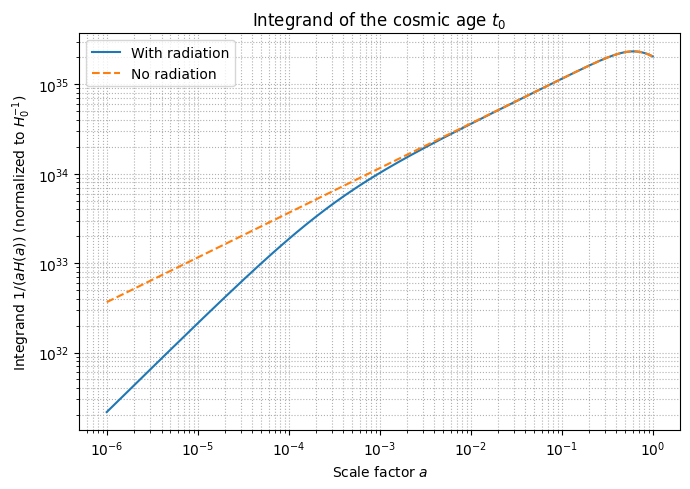
\includegraphics[width=0.75\linewidth]{Appendix_Fig_A1_t0_integrand_updated.png}
    \caption{
    Integrand of the cosmic age $t_0$ as a function of scale factor $a$, 
    shown with (solid line) and without (dashed line) the radiation term.
    The radiation contribution is significant only for $a \lesssim 10^{-4}$,
    indicating that the late-time expansion dominates the total age integral.
    Integration of this curve gives $t_0 \simeq 13.66$~Gyr for the SFT baseline parameters.}
    \label{fig:appA1}
\end{figure}


\textit{\textbf{\underline{Figure \ref{fig:appA1} \textit{Integrand of cosmic age $t_0$} Interpretation:}}}
The integrand $1/(aH(a))$ highlights that radiation (dashed curve) contributes appreciably only for $a\lesssim10^{-4}$, confirming that most of the age of the Universe accumulates during the matter– and dark–energy–dominated epochs. Integrating the curve yields $t_0\simeq13.66$ Gyr for the SFT baseline.


%%%%%%%%%%%%%%%%%%%%%%%%%%%%%%%%%%%%%%%%%%%%%%%%%%%%%%%%%%%%%%%%%%%%%%%%%%%%%%%%%%%%%%%%%%%%%%%%%%%%%%

\subsection{Figure \ref{fig:SFT_SN_residuals_updated}: \textit{SFT--$\Lambda$CDM supernova residuals $\Delta\mu(z)$.}}

\begin{figure}[H]
\centering
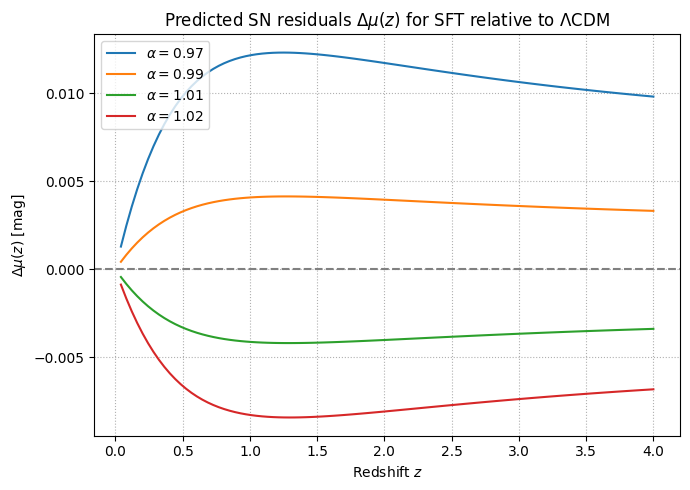
\includegraphics[width=0.75\linewidth]{SFT_SN_residuals_updated.png}
\caption{
Predicted supernova residuals $\Delta\mu(z) \equiv \mu_{\mathrm{SFT}}(z) - \mu_{\Lambda\mathrm{CDM}}(z)$ 
for several values of the dark-energy evolution parameter $\alpha$.
Phantom-like cases ($\alpha=0.97,\,0.99$) produce positive residuals
(larger distance moduli), while quintessence-like cases
($\alpha=1.01,\,1.02$) yield negative residuals
(smaller distance moduli) at high redshift.
For $\alpha=1$, the SFT curve coincides exactly with $\Lambda$CDM ($\Delta\mu=0$).  
The predicted offsets of $0.02$–$0.06$~mag at $z\!\lesssim\!4$ lie within 
the sensitivity of LSST, Roman, and DESI precision cosmology surveys, 
offering a direct test of the SFT dark-energy law $\rho_{\rm DE}(a)=\rho_{{\rm DE},0}a^{3(1-\alpha)}$.
}
\label{fig:SFT_SN_residuals_updated}
\end{figure}


\textit{\underline{\textbf{Figure \ref{fig:SFT_SN_residuals_updated} \textit{SFT--$\Lambda$CDM supernova residuals $\Delta\mu(z)$ }Interpretation:}}}
Phantom-like cases ($\alpha<1$) produce positive residuals
($\Delta\mu>0$), corresponding to larger luminosity distances, while
quintessence-like cases ($\alpha>1$) produce negative residuals
($\Delta\mu<0$), corresponding to smaller luminosity distances. The
residuals reach approximately $\pm(0.02$--$0.06)$ mag by
$z\simeq2$--$4$. These conditional responses provide an observational
test of the SFT dark-energy law
$\rho_{\rm DE}(a)=\rho_{\rm DE,0}a^{3(1-\alpha)}$.

%%%%%%%%%%%%%%%%%%%%%%%%%%%%%%%%%%%%%%%%%%%%%%%%%%%%%%%%%%%%%%%%%%%%%%%%%%%%%%%%%%%%%%%%%%%%%%%%%%%%%%%

\subsection{Figure \ref{fig:DeltaMu_panels}: \textit{Fractional densities $\Omega_m(z)$ and $\Omega_{\rm DE}(z)$ for SFT and $\Lambda$CDM}}

\begin{figure}[H]
\centering
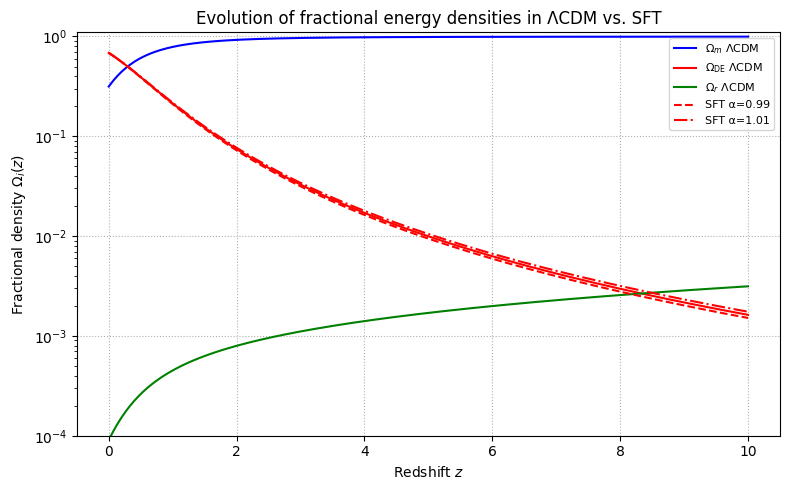
\includegraphics[width=0.75\linewidth]{DeltaMu_panels.png}
\caption{
Predicted SN residuals $\Delta\mu(z)$ for SFT relative to $\Lambda$CDM.
Left: phantom-like ($\alpha=0.97,0.99$).
Right: quintessence-like ($\alpha=1.01,1.02$). 
For $\alpha=1$, the curve coincides with $\Lambda$CDM ($\Delta\mu=0$).
}
\label{fig:DeltaMu_panels}
\label{fig:Omega_evolution_LCDM_SFT_z10}
\end{figure}


\textit{\textbf{\underline{Figure \ref{fig:DeltaMu_panels} \textit{Fractional densities $\Omega_m(z)$ and $\Omega_{\rm DE}(z)$ for SFT and $\Lambda$CDM} Interpretation:}}}
The evolution of $\Omega_m(z)$, $\Omega_{\rm DE}(z)$, and $\Omega_r(z)$ illustrates that SFT tracks $\Lambda$CDM at early times but deviates gently at $z\lesssim2$. For $\alpha=0.99$, dark energy declines more steeply (slower acceleration), while for $\alpha=1.01$ it grows slightly faster. These percent–level shifts are measurable with Euclid and DESI $H(z)$ and growth–rate data.

%=====================================
\begin{table}[h!]
\centering
\small
\setlength{\tabcolsep}{5.5pt}
\renewcommand{\arraystretch}{1.15}
\caption{
\textbf{Companion table to Fig.~\ref{fig:DeltaMu_panels}.}
Fractional densities $\Omega_m(z)$ and $\Omega_{\rm DE}(z)$ at benchmark redshifts 
for $\Lambda$CDM ($\alpha=1$) and SFT variants ($\alpha=0.99,\,1.01$),
computed using the SFT baseline:
$H_0=68.05~{\rm km\,s^{-1}\,Mpc^{-1}}$, 
$\Omega_{m,0}=0.315$, 
$\Omega_{r,0}=9.034\times10^{-5}$, 
and $\Omega_{\rm DE,0}=0.68491$.
Radiation is included in the background but contributes $\lesssim0.2\%$ 
for $z\le5$ and is omitted from the table body for readability.
}
\label{tab:Omega_benchmarks_companion}
\begin{tabular}{lcccccccc}
\toprule
\multirow{2}{*}{Model} &
\multicolumn{2}{c}{$z=1$} &
\multicolumn{2}{c}{$z=2$} &
\multicolumn{2}{c}{$z=3$} &
\multicolumn{2}{c}{$z=5$} \\
\cmidrule(lr){2-3}\cmidrule(lr){4-5}\cmidrule(lr){6-7}\cmidrule(lr){8-9}
 & $\Omega_m$ & $\Omega_{\rm DE}$ 
 & $\Omega_m$ & $\Omega_{\rm DE}$ 
 & $\Omega_m$ & $\Omega_{\rm DE}$ 
 & $\Omega_m$ & $\Omega_{\rm DE}$ \\
\midrule
$\Lambda$CDM ($\alpha=1$)      & 0.786 & 0.214 & 0.925 & 0.074 & 0.966 & 0.033 & 0.988 & 0.010 \\
SFT, $\alpha=0.99$ (phant.)    & 0.789 & 0.210 & 0.927 & 0.072 & 0.967 & 0.032 & 0.989 & 0.009 \\
SFT, $\alpha=1.01$ (quint.)    & 0.782 & 0.217 & 0.922 & 0.077 & 0.965 & 0.034 & 0.988 & 0.010 \\
\bottomrule
\end{tabular}
\end{table}

\paragraph{Interpretation of Table~\ref{tab:Omega_benchmarks_companion}.}
This table summarizes the evolution of the fractional energy densities
$\Omega_m(z)$ and $\Omega_{\rm DE}(z)$ in $\Lambda$CDM and SFT
cosmologies using the updated 2025 baseline parameters. The only difference between the models is the SFT
dark-energy evolution index $\alpha$.

For $\alpha=0.99$ (phantom-like), the dark-energy density decreases
slightly with increasing redshift, corresponding equivalently to an
increase toward the future. This yields a marginally lower
$\Omega_{\rm DE}(z)$ than in $\Lambda$CDM at positive redshift.
For $\alpha=1.01$ (quintessence-like), the dark-energy density increases
slightly with increasing redshift, corresponding equivalently to a
decrease toward the future, and yields a marginally higher
$\Omega_{\rm DE}(z)$ than in $\Lambda$CDM at positive redshift.

These percent-level deviations are subtle but potentially measurable by
next-generation surveys such as DESI, Euclid, and LSST, providing a
direct observational test of the SFT dark-energy evolution law

\[
\rho_{\rm DE}(a)
=
\rho_{\rm DE,0}\,a^{3(1-\alpha)}.
\]

%%%%%%%%%%%%%%%%%%%%%%%%%%%%%%%%%%%%%%%%%%%%%%%%%%%%%%%%%%%%%%%%%%%%%%%%%%%%%%%%%%%%%%%%%%%%%%%%%%%%%%%%

\subsection{Figure \ref{fig:H_ratio_SFT_LCDM}: \textit{Expansion-rate deviation $H_{\mathrm{SFT}}/H_{\Lambda\mathrm{CDM}}-1$.}}

\begin{figure}[H]
\centering
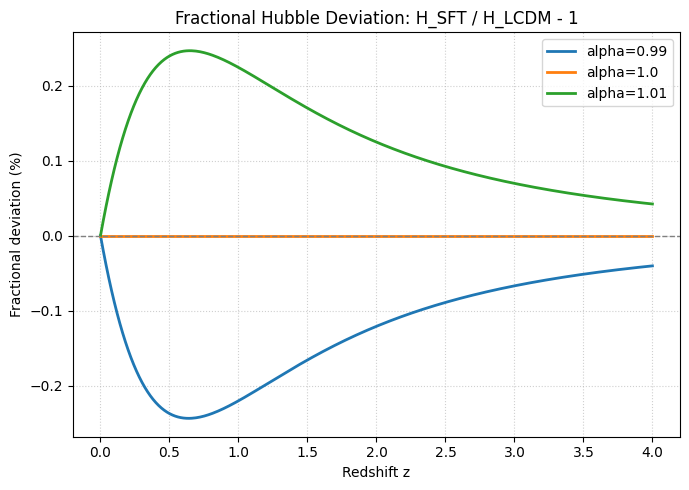
\includegraphics[width=0.75\linewidth]{H_ratio_SFT_LCDM.png}
\caption{
Fractional deviation of the expansion rate 
$H_{\mathrm{SFT}}(z)/H_{\Lambda\mathrm{CDM}}(z)-1$ 
for $\alpha=0.99$, $1.00$, and $1.01$.
Departures of $\pm(1$--$2)\%$ occur by $z\simeq2$,
providing a direct geometric probe of the SFT parameter $\alpha$.
Future redshift–drift and BAO–$H(z)$ measurements (ELT, DESI, Euclid)
can test this signature with percent-level precision.}
\label{fig:H_ratio_SFT_LCDM}
\end{figure}


\textit{\textbf{\underline{Figure \ref{fig:H_ratio_SFT_LCDM} \textit{Expansion-rate deviation $H_{\mathrm{SFT}}/H_{\Lambda\mathrm{CDM}}-1$.} Interpretation:}}}
The ratio $H_{\rm SFT}/H_{\Lambda{\rm CDM}}-1$ departs by $\pm(1$–$2)\%$ by $z\simeq2$ for $|\alpha-1|\simeq0.01$. Precision redshift–drift and BAO measurements from ELT, DESI, and Euclid can resolve these deviations directly, offering a purely geometric test of the SFT confinement relation.


%%%%%%%%%%%%%%%%%%%%%%%%%%%%%%%%%%%%%%%%%%%%%%%%%%%%%%%%%%%%%%%%%%%%%%%%%%%%%%%%%%%%%%%%%%%%%%%%%%%%%%%%

\subsection{\textbf{Figure \ref{fig:siren_SFT_LCDM}}:
\textit{Standard-siren distance residual relative to $\Lambda$CDM.}}

\begin{figure}[H]
\centering
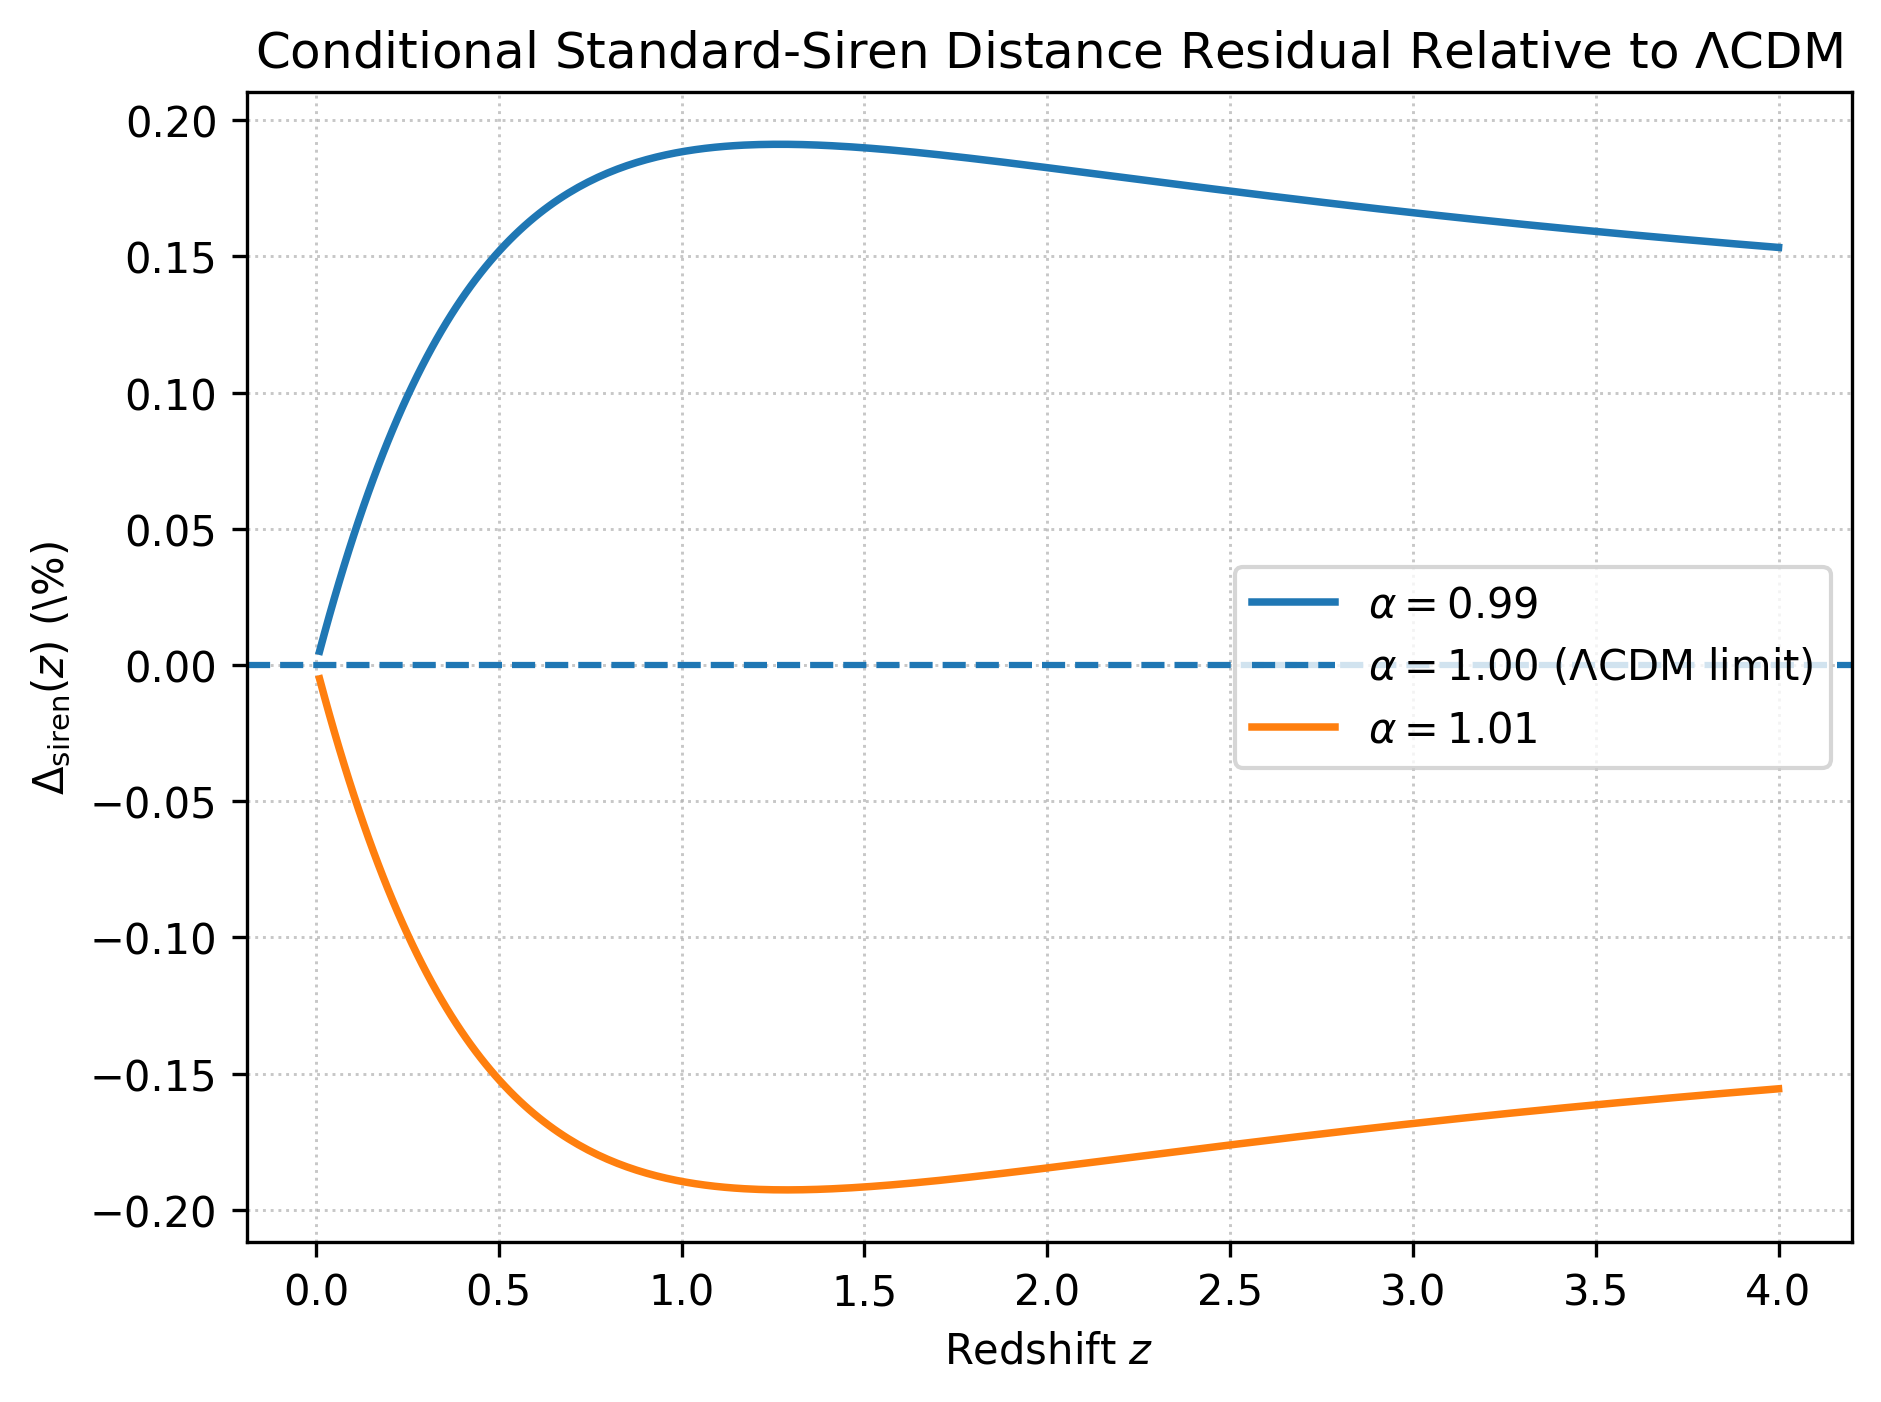
\includegraphics[width=0.75\linewidth]
{standard_siren_SFT_LCDM_residual.png}
\caption{
Conditional standard-siren luminosity-distance residual
\[
\Delta_{\rm siren}(z)
=
\frac{d_L^{\rm SFT}(z)}
     {d_L^{\Lambda{\rm CDM}}(z)}
-1
\]
for $\alpha=0.99$ and $\alpha=1.01$.
For $|\alpha-1|=0.01$, the residual reaches approximately
$0.2\%$ in magnitude around $z\sim1$--$2$.
The effect arises from the different background expansion histories,
not from modified gravitational-wave propagation.
}
\label{fig:siren_SFT_LCDM}
\end{figure}

\textit{\underline{\textbf{
Figure \ref{fig:siren_SFT_LCDM}:
\textit{Standard-siren distance residual relative to $\Lambda$CDM.}
Interpretation:}}}
For representative values $\alpha=0.99$ and $\alpha=1.01$, the SFT
background produces opposite-sign luminosity-distance residuals of
order $0.2\%$ relative to the $\Lambda$CDM background. Gravitational
waves and electromagnetic radiation retain the same luminosity
distance within each fixed cosmology. Standard sirens therefore test
the SFT background expansion rather than a modified tensor-propagation
law.


%%%%%%%%%%%%%%%%%%%%%%%%%%%%%%%%%%%%%%%%%%%%%%%%%%%%%%%%%%%%%%%%%%%%
\subsection{Supernova residuals $\Delta\mu(z)$ for SFT indices $\alpha$}

\begin{table}[H]
\centering
\small
\setlength{\tabcolsep}{5pt}
\renewcommand{\arraystretch}{1.15}
\caption{
Benchmark supernova distance--modulus residuals 
$\Delta\mu(z)=\mu_{\rm SFT}(z)-\mu_{\Lambda{\rm CDM}}(z)$ 
at representative redshifts for SFT indices $\alpha$,
computed with the SFT parameters:
$H_0=68.05~{\rm km\,s^{-1}\,Mpc^{-1}}$, 
$\Omega_{m,0}=0.315$, 
$\Omega_{r,0}=9.034\times10^{-5}$, 
$\Omega_{\rm DE,0}=0.68491$,
and $M_{r,0}=2.79344\times10^{50}\ {\rm kg}$.
Changing $H_0$ rescales both models equally, so it cancels in $\Delta\mu$.
Positive values indicate larger SFT distance moduli than in
$\Lambda$CDM and therefore slightly fainter inferred supernovae at fixed
redshift, while negative values correspond to smaller distance moduli
and slightly brighter inferred supernovae.
}
\label{tab:SN_residuals}
\begin{tabular}{c c c}
\toprule
$z$ & $\alpha$ & $\Delta\mu$ [mag] \\
\midrule
0.5 & 0.97 & $+0.018$ \\
    & 1.01 & $-0.007$ \\
    & 1.02 & $-0.015$ \\
\hline
1.0 & 0.97 & $+0.037$ \\
    & 0.99 & $+0.015$ \\
    & 1.01 & $-0.015$ \\
    & 1.02 & $-0.031$ \\
\hline
1.5 & 0.97 & $+0.048$ \\
    & 0.99 & $+0.020$ \\
    & 1.01 & $-0.020$ \\
    & 1.02 & $-0.041$ \\
\hline
2.0 & 0.97 & $+0.054$ \\
    & 0.99 & $+0.022$ \\
    & 1.01 & $-0.022$ \\
    & 1.02 & $-0.045$ \\
\hline
3.0 & 0.97 & $+0.060$ \\
    & 0.99 & $+0.025$ \\
    & 1.01 & $-0.025$ \\
    & 1.02 & $-0.050$ \\
\hline
4.0 & 0.97 & $+0.063$ \\
    & 0.99 & $+0.026$ \\
    & 1.01 & $-0.026$ \\
    & 1.02 & $-0.052$ \\
\bottomrule
\end{tabular}
\end{table}


\noindent\textbf{Interpretation of Table~\ref{tab:SN_residuals}.}
Phantom-like cases, $\alpha<1$, yield $\Delta\mu>0$, corresponding to
slightly larger luminosity distances and fainter inferred supernovae
relative to $\Lambda$CDM. Quintessence-like cases, $\alpha>1$, yield
$\Delta\mu<0$, corresponding to slightly smaller luminosity distances
and brighter inferred supernovae.

The offsets grow smoothly with redshift, reaching approximately
$\pm(0.02$--$0.06)$ mag by $z\simeq4$. These amplitudes are conditional
responses to the specified values of $\alpha$, rather than parameter-free
predictions of the minimal SFT closure condition.

They provide an observational test of the phenomenological SFT
dark-energy evolution law
\[
\rho_{\rm DE}(a)
=
\rho_{{\rm DE},0}a^{3(1-\alpha)}.
\]

%%%%%%%%%%%%%%%%%%%%%%%%%%%%%%%%%%%%%%%%%%%%%%%%%%%%%%%%%%%%%%%%%%%%%%%%%%%

\section*{Acknowledgements}

The author used AI-assisted tools, including large language models,
for proofreading, LaTeX formatting, editorial refinement, and assistance
in checking the internal consistency and presentation of the manuscript.
The underlying theoretical framework, scientific hypotheses, original
derivations, numerical methodology, interpretation of results, and final
scientific conclusions are the responsibility of the author.

%%%%%%%%%%%%%%%%%%%%%%%%%%%%%%%%%%%%%%%%%%%%%%%%%%%%%%%%%%%%%%%%%%%%
%%%%%%%%%%%%%%%%%%%%%%%%%%%%%%%%%%%%%%%%%%%%%%%%%%%%%%%%%%%%%%%%%%%%
\section*{Data and Code Availability}
\label{sec:data_code}

All numerical computations, figure-generation scripts, and tabulated datasets 
used in this work are publicly available and reproducible.

\begin{itemize}
\item \textbf{Zenodo (archival, citable version):}  
\url{https://doi.org/10.5281/zenodo.17455433}

\item \textbf{GitHub repository:}
\href{https://github.com/joshuaegbon7-sketch/Spacefield-Transformation-Paper-1/tree/SFT-1}
{Spacefield Transformation Paper 1 Repository}
\footnote{\url{https://github.com/joshuaegbon7-sketch/Spacefield-Transformation-Paper-1/tree/SFT-1}}

\end{itemize}

The Zenodo DOI \texttt{10.5281/zenodo.17455433} represents all versions of the 
dataset and always resolves to the latest archived release. It should be used 
for formal citation of the computational materials associated with this work.

The Zenodo archive provides a permanent, versioned snapshot corresponding to 
the results presented in this paper, including:
\begin{itemize}
\item all figures and tables used in the main text and supplementary numerical diagnostics;
\item all tables and benchmark datasets;
\item Python scripts used for cosmological integrations and plotting.
\end{itemize}

The GitHub repository provides direct access to the same codebase and materials 
used in this work.

\newpage
\bibliographystyle{unsrt}
\bibliography{SFT_Paper1_References}


\end{document}








